\documentclass[final,italian,titlepage,listoffigures,listoflistings,fullbib,openright,a4paper,nobibtex]{tesi}

\usepackage{graphicx}

\usepackage[LGR,T1]{fontenc}
\def\sfdefault{cmss}

\usepackage{tabularx}
\usepackage{calc}
\usepackage{comma}
\usepackage{lscape}
\usepackage[all]{xy}
\usepackage{thumbpdf}
\usepackage{enumerate}
\usepackage{dsfont}
\usepackage[bf]{caption}
\makeatletter
\let\comma\@commaform
\makeatother
\hyphenation{vi-sua-liz-za-bi-li
			 mo-di-fi-ca-te
			 ge-ne-ra-to
			 va-lo-ri
			 si-mi-la-ri-t�
			 ge-ne-ra-re
			 fram-men-ta-rie-t�
			 piat-ta-for-ma
			 re-in-ge-gne-riz-za-zio-ne
			 qual-sia-si
			 initialize-Method
			 piat-ta-for-ma
			 mo-del-lo
			 per-so-na-liz-za-ta}

\begin{document}

\selectlanguage{italian}

\author{Niccol� {\sc Olivieri Achille}}
\title{Realizzazione di un sistema di raccomandazione in Matlab}
\anno{2009/2010}
\matricola{724811}
\relatore{Prof. Paolo {\sc Cremonesi}}
\correlatore{Prof. Roberto {\sc Turrin}}

\universita[./img/poli]
	{Politecnico di Milano}
	{Facolt� di Ingegneria dell'Informazione}
	{Corso di laurea in Ingegneria Informatica}

\makeatletter
\ifpdf
	\hypersetup{pdftitle={\@title}
			   ,pdfsubject={Tesi di Laurea Specialistica}
			   ,pdfauthor={\@author}}
\fi
\makeatother

% Macro per aggiungere le migliaia
\makeatletter
\let\comma\@commaform
\makeatother

% Environment for inline code (monoscpaced font)
\newcommand{\cod}[1]{\texttt{#1}}

% Environment for inline memory address
\newcommand{\addr}[1]{\footnotesize{\texttt{#1}}}

% Redefine \emph to avoid \xspace issue
\renewcommand{\emph}[1]{\bgroup\em #1\egroup}

% Environment for initial italian abstract
\renewenvironment{abstract}{
  \def\abstract@title{Riassunto della tesi}
  \chapter*{\abstract@title}
   \addcontentsline{toc}{chapter}{\abstract@title}
  \renewcommand\thepage{\roman{page}}
  \onehalfspacing
}{}

% Environment for two listings
\newenvironment{twolistings}[2]{%
  \begingroup%
  \tabskip=0pt%
  \setbox2\vbox\bgroup%
    \halign\bgroup%
      \vrule\hbox{\vbox{\hsize=#1##}}~\vrule~ & %
            \hbox{\vbox{\hsize=#2##}}~\vrule\cr %
      \vskip1em}{%
      \cr%
    \egroup%
  \egroup%
  \vbox{\hrule\box2\hrule}%
  \endgroup%
}

% Macros for images
\newcommand{\myfigure}[6][]{%
  \begin{figure}[h!t]%
    \centering
    \vspace{#5}
    \includegraphics[#1]{#2}%
    \vspace{#6}
    \caption{#3}%
    \label{#4}%
  \end{figure}%
} 

\newcommand{\myfiguree}[7][]{%
  \begin{figure}[h!t]%
    \centering
    \vspace{#5}
    \includegraphics[#1]{#2}%
    \vspace{#6}
    \caption[#7]{#3}%
    \label{#4}%
  \end{figure}%
} 

\newcommand{\mysinglefigure}[6][]{%
  \begin{figure}[p!]%
    \centering
    \vspace{#5}
    \includegraphics[#1]{#2}%
    \vspace{#6}
    \caption{#3}%
    \label{#4}%
  \end{figure}%
} 


\newcommand{\mycode}[4]{%
 \begin{figure}[ht!]%
  \begin{minipage}[c]{1\textwidth}%
   {#4
     \verbatiminput{#1}%
   }
  \end{minipage}%
  \caption{#2}%
  \label{#3}%
 \end{figure}
}

\newcommand{\mytwocode}[9]{%
  \begin{figure}[ht!]%
     \vspace{0.5cm}%
     \subfigure[#2]{%
       \label{#3}%
       \begin{minipage}[c]{0.5\textwidth}%
	     \centering%
           {#4
             \verbatiminput{#1}%
           }%
  	     \vspace{0.2cm}%
       \end{minipage}}%
     \hspace{0.2cm}%
     \subfigure[#6]{%
       \label{#7}%
       \begin{minipage}[c]{0.5\textwidth}%
	     \centering%
           {#4
             \verbatiminput{#5}%
           }%
  	     \vspace{0.2cm}%
       \end{minipage}}%
     \hspace{0.2cm}%
     \caption{#8}%
     \label{#9}%
   \end{figure}%
}%

\newcommand{\mytwofracode}[9]{%
  \begin{figure}[ht!]%
     \vspace{0.5cm}%
     \subfigure[#2]{%
       \label{#3}%
       \begin{minipage}[c]{0.4\textwidth}%
	     \centering%
           {#4
             \verbatiminput{#1}%
           }%
  	     \vspace{0.2cm}%
       \end{minipage}}%
     \hspace{0.2cm}%
     \subfigure[#6]{%
       \label{#7}%
       \begin{minipage}[c]{0.6\textwidth}%
	     \centering%
           {#4
             \verbatiminput{#5}%
           }%
  	     \vspace{0.2cm}%
       \end{minipage}}%
     \hspace{0.2cm}%
     \caption{#8}%
     \label{#9}%
   \end{figure}%
}%

\newtextcommand{\vod}{\textsc{VoD}}
\newtextcommand{\iptv}{\textsc{IPTv}}

\newtextcommand{\icm}{\textsc{ICM}}
\newtextcommand{\urm}{\textsc{URM}}
\newtextcommand{\bow}{\textsc{BoW}}
\newtextcommand{\csv}{\textsc{CSV}}

%%%%%%%%%%%%%%%%%%%%%%%%%%%%%%%%%%%%%%%%%%%%%%%%%%%%%%%%%%%%%%%%%%%%%%%%%%
%%								FRONTMATTER								%%
%%%%%%%%%%%%%%%%%%%%%%%%%%%%%%%%%%%%%%%%%%%%%%%%%%%%%%%%%%%%%%%%%%%%%%%%%%

\frontmatter

\normalfont

\thispagestyle{empty}
\vspace{17cm}

%\large
\begin{flushright}
\itshape{ Alla mia famiglia}
\end{flushright}


\pagenumbering{Roman}
\pagestyle{plain}

\begin{sommario}

Al giorno d'oggi la sempre pi� vasta domanda di contenuti audiovisivi specifici sta obbligando i vari distributori di servizi quali \corsivo{Video on Demand} e \corsivo{IP Television} a utilizzare algoritmi di raccomandazione per aiutare l'utente nella fase di scelta.

Nel corso degli anni � stata creata una gran quantit� di algoritmi in grado di effettuare una raccomandazione e quest'enorme offerta ha reso la vita incredibilmente difficile a tutti coloro che han dovuto tenere aggiornate le varie piattaforme di suggerimenti e test sull'efficacia degli stessi. Ed � proprio questa fase di test che pi� preoccupa in quanto � computazionalmente molto impegnativa. 

La ricerca della \corsivo{semplificazione} e dell'\corsivo{estendibilit�} � l'obiettivo che ci si pone in questa tesi: per un momento si vuole interrompere la ricerca di nuovi algoritmi o nuove metodologie di test, in favore di una reingegnerizzazione di tutto il sistema di raccomandazione, rendendolo pi� leggibile anche ai non addetti ai lavori e soprattutto facilmente estendibile per i nuovi algoritmi che verranno sicuramente ideati negli anni a venire.

Il tutto viene realizzato appoggiandosi a quell'incredibile strumento che � Matlab, in modo da tralasciare l'ideazione di strutture dati complesse, lasciando tutta la complessit� al linguaggio di programmazione. Matlab, infatti, implementa delle funzioni in grado di calcolare in maniera molto rapida complesse strutture matematiche, che altrimenti richiederebbero una fase di programmazione molto pi� lunga.

\end{sommario}
\begin{ringraziamenti}

Che dire, anche la laurea specialistica � conclusa, e questo lavoro di tesi segna la fine della mia avventura universitaria. Ripenso a tutti coloro che hanno contribuito a questo ""successo'' ed � con grande piacere che li voglio ricordare.

In primis mi sento di \corsivo{dover} ringraziare i miei compagni di peripezie, \grassetto{Cecio}, \grassetto{Luca} e \grassetto{Andre}, in quanto mi hanno sopportato e supportato in tutti questi anni dentro e fuori le mura del Poli. Inutile dire che senza le giornate di studio collettivo ""alba-tramonto'' non avrei neanche raggiunto il traguardo della laurea triennale. Un ringraziamento particolare va senz'altro a Cecio che ci ha sempre fornito un pasto caldo, una casa calda (soprattutto in estate) e tanta elettricit� per le sedute notturne! Ma non voglio dimenticare il sette-e-mezzo a Cervinia (e soprattutto quel che successe dopo) o gli \corsivo{invisibili} di Ponza (Andre, dobbiamo ancora spiegarti come ci si ferma!). Ora basta, almeno per un paio di mesi (nel caso di Cecio \corsivo{anni}) non voglio pi� vedervi!

Il secondo grazie va senz'altro alla mia famiglia, a \grassetto{mia madre}, che seppur con minacce e grida ha sempre dimostrato fiducia nelle mie capacit� (sar� stato vero amore o sfrenato desiderio di non dovermi pi� mantenere?), a \grassetto{mia nonna} che pur di vedermi ingegnere mi ha spronato e blandito con lacrime e regali. Grazie anche a \grassetto{mio padre} che ha desiderato con tutte le sue forze questa laurea e che purtroppo non � qui a condividere la mia gioia, e ai \grassetto{miei fratelli} che si sono talmente impegnati a rendermi la vita impossibile in casa che ho considerato la laurea e il conseguente cambio di vita come l'affrancamento dalla caotica vita familiare.

Un ringraziamento particolarissimo va al \grassetto{Professor Cremonesi}, che mi ha fatto appassionare ai sistemi di raccomandazione e che � riuscito a trovarmi una tesi ""adatta'' alle mie esigenze di tempi stringati, e a \grassetto{Roby} che, votato alla santit�, � riuscito a sopportarmi in questi mesi su Skype!

Okey, ultimati i ringraziamenti ""obbligati'' passiamo ora a tutte le persone che, oltre ai summenzionati tre grandi amici Dott. Ing., mi sono state vicine in questi anni. Voglio senz'altro iniziare dalla mia cugina adottiva, \grassetto{Ko}, che con grande intuizione � sempre riuscita a farmi passare le notti in giro quando ero sotto esami e a farmi perdere tempo su MSN quando dovevo studiare\ldots ogni tanto mi chiedo perch� non abbia gi� cestinato il suo indirizzo email e il suo numero di telefono! Deve esserci una spiegazione freudiana\ldots

Ecco ora la mia famiglia allargata, le sorelline \grassetto{Robi} e \grassetto{Ro} che son riuscite a mantenermi sempre sulla retta via distraendomi dallo studio e facendomi spesso dimenticare i miei doveri: vogliamo ricordare una certa vacanza e un certo carrello della spesa (Robi) oppure le telefonate di mezzogiorno dal Poli (Ro)?

E come dimenticare i ""colleghi'', gli altri \corsivo{furbacchioni} che insieme a me hanno scelto il Poli come propria morte intellettuale: \grassetto{Zoid}, \grassetto{Tig}, \grassetto{Patrick}, \grassetto{Pan}, \grassetto{Monzio}, \grassetto{Axel}, \grassetto{Max}, \grassetto{Botta} e tutti gli altri che in questi anni mi han sempre spronato ad arrivare alla fine (""se ce l'ha fatta lui ce la posso fare pure io''!!).

Ci sono poi tutti gli amici con cui si � condivisa buona parte del (poco?) tempo in cui non si studiava: a cominciare da tutti coloro che ho conosciuto tramite internet e che sono un punto fermo nei miei momenti di svago: dai pi� recenti: \grassetto{Gossip}, \grassetto{Nilu}, \grassetto{Vergat}, \grassetto{Kim}, \grassetto{Chri}, \grassetto{i Dadi}, \grassetto{Khitty}, \grassetto{Death}, \grassetto{Galac}, \grassetto{Khoruss}, \grassetto{Eliset}, \grassetto{Chime} e \grassetto{i sanremesi}, ma in fondo in fondo anche Amy, Moghe, Ares, Taki, It, Bio, Ayaion, Peppe, Marco, Ste, Maicol ecc ecc per arrivare a \grassetto{la Fede}, \grassetto{Vi�}, \grassetto{Laz}, \grassetto{il Fra}, \grassetto{la Vale}, \grassetto{il Deb}, \grassetto{Carmine}, \grassetto{Marco}, \grassetto{Khai}, \grassetto{Arwin} e a tutto il vecchio (vecchissimo) gruppo dei GDR.

Ultimi ma non ultimi tutti i cretini del Fashion che son sempre riusciti a convincermi a fare serata il venerd� sera (e anche molti sabati): \grassetto{i fratellini}, \grassetto{Edo}, \grassetto{Gerry}, \grassetto{tutti gli ex-Zacca} (siete troppi!) e tutti gli altri che in questi anni han popolato il nostro ritrovo fisso!

E anche a tutti gli altri che ora sto omettendo ma che han popolato il mio mondo di studente poco modello ma sufficiente coscienzioso, un grazie di cuore da chi oggi � consapevole di chiudere un capitolo piacevole della sua vita per aprirne un altro ben pi� oneroso.

\end{ringraziamenti}

%%%%%%%%%%%%%%%%%%%%%%%%%%%%%%%%%%%%%%%%%%%%%%%%%%%%%%%%%%%%%%%%%%%%%%%%%%
%%								MAINMATTER								%%
%%%%%%%%%%%%%%%%%%%%%%%%%%%%%%%%%%%%%%%%%%%%%%%%%%%%%%%%%%%%%%%%%%%%%%%%%%

\mainmatter

\chapter{Introduzione}
\label{c:int}

Servizi di e-commerce e di Internet Television (pi� brevemente \iptv) hanno in comune un grandissimo database, da poter offrire all'utente, di oggetti acquistabili nel caso di portali di e-commerce e di contenuti audiovisivi visualizzabili attraverso il Video on Demand (pi� brevemente \vod) per quanto riguarda le televisioni sul web. E se questa particolarit� pu� sembrare un vantaggio, c'� anche un retro della medaglia, una faccia che questi provider si trovano a dover affrontare ogni giorno in modo sempre pi� disperato: informare l'utente dell'esistenza di questo enorme database, rendendone semplice la consultazione e la ricerca. Ma cerchiamo di capire meglio di cosa si sta parlando: nel caso si sia mai visitato un portale di e-commerce con l'intento di fare acquisti, si sar� poi notato che il sistema, una volta visualizzata la scheda di un oggetto, suggerisce altri oggetti che potrebbero interessare, in quanto ricercati o visualizzati da chi ha acquistato prima di noi. Senza troppi giri di parole questa � una semplice \grassetto{raccomandazione}, in quanto il sito ha in memoria lo storico dei suoi clienti e lo mette a nostra disposizione per consigliarci un ulteriore oggetto nella speranza che ci possa in qualche modo interessare.

Similmente funziona l'\iptv. In questo caso per� si ha a che fare con risorse audiovisive che quindi devono sottostare ai gusti dell'utente. del quale il sistema registra lo storico\nota{In seguito esamineremo meglio cosa si intende per "storico"} per poi suggerire la visione di un contenuto piuttosto che di un altro. Ma � proprio in questo momento che subentra l'ostacolo pi� grande, tipico proprio dei servizi di \iptv e \vod: il sistema di interfacciamento � infinitamente pi� semplice e meno funzionale di quello che si ha a disposizione quando l'utente si mette davanti al computer, ora � un semplice telecomando che ci permette di controllare il flusso di dati. Scorrere quindi attraverso pagine e pagine di contenuti pu� risultare lungo, ma soprattutto fastidioso per l'utente che desidera avere risultati veloci. 

Da questa semplice panoramica � facilmente intuibile l'utilit� dei \grassetto{sistemi di raccomandazione}: sono in grado di suggerire a real time un numero limitato ma incredibilmente specifico di contenuti altamente \corsivo{personalizzati}. Tutto ci� � ovviamente volto a rendere sempre pi� soddisfatto l'utente e, conseguentemente, incrementare le vendite dei prodotti.

Un sistema di raccomandazione � in grado di consigliare determinati contenuti in base a:
\begin{itemize}
	\item il \corsivo{profilo utente}, ovvero le singole preferenze, espresse in modo pi� o meno esplicito;
	\item le caratteristiche dei contenuti stessi (\corsivo{modello degli item}).
\end{itemize}

Il profilo utente � lo storico delle interazioni tra l'utente e i contenuti. Vengono memorizzate sia le visualizzazioni di un determinato oggetto del catalogo, sia la valutazione (avvenuta quindi in modo esplicito) che gli � stata attribuita. In questo modo si crea una sorta di ""carta di identit�'' dell'utente.

Il modello dei vari item riguarda le caratteristiche dei contenuti disponibili a catalogo. In base all'algoritmo scelto queste caratteristiche riguarderanno il contenuto dell'item oppure le preferenze indicate dalla comunit� degli utenti. Nel primo caso parleremo di algoritmi \corsivo{Content-Based}, nel secondo di algoritmi \corsivo{Collaborativi}.

Fine ultimo del sistema di raccomandazione � restituire una lista di N valori (per questo chiamata \grassetto{lista Top-N} in cui N solitamente � 10). Questa lista pu� essere anche filtrata in modo da controllarne la dinamicit� in vari momenti.

In questa tesi si vuole quindi creare una piattaforma in grado di utilizzare i sistemi di raccomandazione non solo per generare i suddetti ""consigli'', ma anche per valutarne la bont� attraverso opportuni test. Il tutto considerando che la tecnologia progredisce e nuovi algoritmi o metodi di test possono essere creati. Proprio per questo sono state studiate e verranno presentate alcune comode API per interfacciarsi ed estendere la piattaforma.

Il lavoro � suddiviso in nove capitoli. \\
Nel Capitolo due viene presentata una breve carrellata dei vari algoritmi utilizzati per le raccomandazioni e le tipologie di dati utilizzate da questi. Ci si soffermer� in particolar modo sulle basi della raccomandazione, in modo da capire poi il processo di reingegnerizzazione.

Nel Capitolo tre saranno trattate le metodologie di test utilizzate, soffermandosi sui risultati che forniscono.

Nel Capitolo quattro si illustrer� lo stato dell'applicazione prima della reingegnerizzazione, trattando in particolar modo la sua frammentazione sia dal punto di vista del codice, sia dal punto di vista dell'ideazione in modo da presentare meglio il problema che si � incontrato. Da qui la necessit� di fermarsi nello sviluppo della piattaforma in modo da riorganizzare il lavoro.

Nel Capitolo quinto si tratter� la reingegnerizzazione vera e propria del sistema, analizzandone la struttura ma soprattutto l'idea di fondo che ne permette l'estendibilit�.

Nel Capitolo sei si studier� la possibile integrazione in un sistema reale, mostrandone i vantaggi e anche dimostrando perch� non possa considerarsi un qualcosa di assolutamente perfetto ed eterno.

Nel Capitolo sette infine si tireranno le somme di quanto � stato studiato, analizzando i possibili sviluppi futuri che l'applicazione pu� avere.
\chapter{Algoritmi di Raccomandazione}
\label{c:algo}

In questo capitolo vengono presentati gli algoritmi usati per effettuare una raccomandazione, introducendo prima cosa sia nella pratica un sistema di raccomandazione e quali dati utilizzi.

\section{Introduzione}
\label{c:algo:intro}

I sistemi di raccomandazione nascono principalmente grazie all'avvento di tecnologie in grado di permettere la fruizione di servizi personalizzati: anche solo una decina di anni fa non si sarebbe mai pensato di poter richiedere al proprio provider un determinato contenuto multimediale. Ora questo � possibile grazie principalmente all'avvento della banda larga, per di pi� il cliente pu� dettare le condizioni e quindi richiedere un servizio sempre migliore.

Ma come avviene questa distribuzione di contenuti? L'\iptv � senz'altro il miglior mezzo per trasmettere questo tipo di richieste, in quanto, essendo parente diretto di Internet, permette ad ogni utente di ricevere un flusso personalizzato. La fruizione pu� quindi avvenire secondo due modalit� differenti, e una terza prevede l'utilizzo delle prime due unite:
\begin{description}
	\item[Streaming] il contenuto viene visionato ""in diretta'', mentre lo si sta scaricando.
	\item[Download] il contenuto � disponibile solo dopo averlo in locale. Questa modalit� � molto comoda in quanto permette di utilizzare protocolli come il Torrent e di accedere alla risorsa anche in un secondo momento, magari in modalit� offline.
	\item[Download Streaming] il contenuto � visionato come in streaming, ma alla fine della visione � disponibile in locale e quindi pu� essere rivisto in un secondo momento.
\end{description}

Questa continua evoluzione delle tecnologie genera un aumento della qualit� richiesta: l'elenco dei titoli disponibili presso i servizi di \vod � in continua crescita, e con esso cresce anche la complessit� della ricerca del contenuto, con la complicazione che il tutto dev'essere controllato tramite un semplice telecomando. Distinguiamo due tipi di ricerca:
\begin{description}
	\item[Information Retrieval (IR)] permette la ricerca del contenuto tramite una parola chiave. Questa ricerca avviene in maniera esatta, quindi i punti di debolezza sono la parola chiave e il sistema, in quanto un contenuto pu� essere stato memorizzato con un nome diverso da quello conosciuto dall'utente. Inoltre, condizione necessaria per la ricerca � la conoscenza, da parte dell'utente, della risorsa stessa, e questo rende la ricerca inutile.
	\item[Information Filtering (IF)] permette un filtraggio delle informazioni in base alle preferenze dell'utente. Questo sistema, nato all'inizio degli anni `90, si sta ritagliando una fetta sempre pi� ampia di mercato in quanto non � necessario l'intervento dell'utente nella fase di ricerca, ma solamente in quella di valutazione del risultato. \`E da questo tipo di ricerca che sono nati i sistemi di raccomandazione, e negli ultimi anni stanno prendendo sempre pi� piede sia in ambito accademico sia in ambito commerciale in quanto si � potuto vedere che consigliare all'utente un oggetto per il quale nutre un certo interesse aumenta le vendite. Questi sistemi prendono come input il \corsivo{profilo utente}, ovvero lo storico dell'utente all'interno del sistema: quali contenuti (in seguito chiamati \corsivo{item}) ha visualizzato, per quali ha espresso una votazione, quali gli sono gi� stati consigliati e cos� via. Inoltre ogni item � descritto tramite un insieme in informazioni (chiamate \corsivo{metadati}) che lo caratterizzano (per esempio un film pu� essere descritto dal regista, dal genere, dagli attori e via dicendo). Grazie a queste, poche, informazioni il sistema � in grado di consigliare nuovi contenuti all'utente, sperando che questi suggerimenti siano di suo gradimento.
\end{description}
Nella trattazione verr� presa in considerazione solamente la ricerca IF in quanto quella IR non � di particolare interesse.

\section{Dati utilizzati}
\label{c:algo:dati}

Gli input utilizzati sono fondamentalmente di due tipi:
\begin{itemize}
	\item La matrice \icm (\grassetto{Item Content Matrix}) che contiene tutti i metadati dei vari item. Le colonne sono quindi gli item (in futuro sar� sempre l'indice \corsivo{j}), mentre le righe sono le differenti parole (vedremo in seguito come si ricavano queste parole) che descrivono le propriet� di cui si vuol tenere traccia. Queste propriet� possono essere inserite o dal sistema (solitamente in fase di aggiunta dell'item) o dagli utenti collaborativamente: in questo modo non ricade tutto sulle spalle dell'azienda che mette a disposizione il servizio. Per contro, le informazioni potrebbero non essere sufficientemente precise in quanto la valutazione dell'utente � sempre soggettiva. Questa matrice viene utilizzata solamente negli algoritmi \corsivo{Content-Based}.
	\begin{figure}
		\begin{center}
			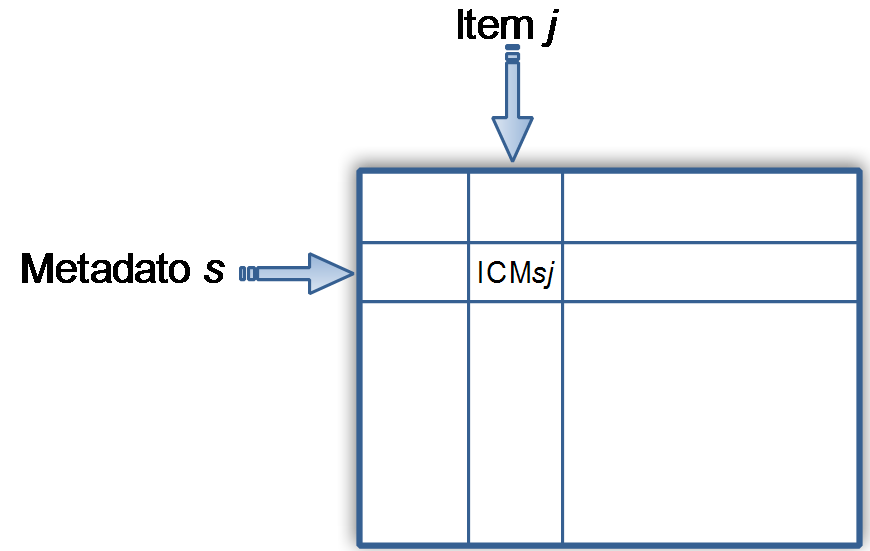
\includegraphics[scale=1]{./img/MatriceICM}
		\end{center}
		\caption{Matrice ICM}
		\label{f:algo:icm}
	\end{figure}
	\item La matrice \urm (\grassetto{User Rating Matrix}) contiene lo storico di tutti gli utenti presenti nel sistema. Le righe rappresentano gli utenti (indicati con l'indice \corsivo{i}), mentre le colonne rappresentano (come visto per la matrice \icm) gli item \corsivo{j}. Ogni elemento della matrice sar� quindi la votazione che l'utente \corsivo{i} ha dato all'item \corsivo{j}. Questa tipologia di matrice si usa negli algoritmi \corsivo{Collaborativi}.
	\begin{description}
		\item[Profilo Utente] � una riga di questa matrice: rappresenta le preferenze di un utente.
	\end{description}
	\begin{figure}
		\begin{center}
			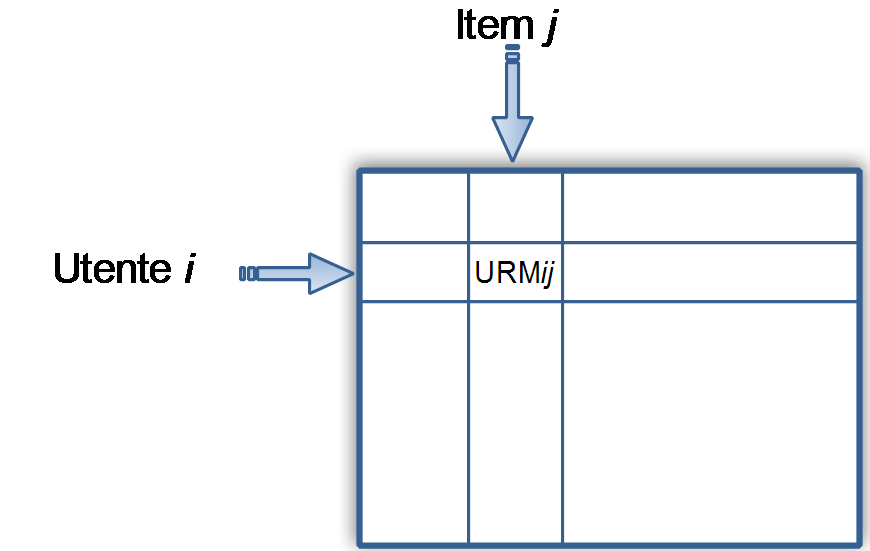
\includegraphics[scale=1]{./img/MatriceURM}
		\end{center}
		\caption{Matrice URM}
		\label{f:algo:urm}
	\end{figure}
\end{itemize}

Come output il sistema di raccomandazione pu� restituire due liste differenti:
\begin{description}
	\item[Individual Scoring] ovvero la votazione che l'utente darebbe ai vari item. In base all'algoritmo scelto questa votazione pu� essere assoluta o relativa.
	\item[Top-N Recommendation] � l'elenco degli N item pi� vicini ai gusti dell'utente. Questa lista viene solitamente creata mettendo in ordine decrescente la lista precedente.
\end{description}

Ma come viene costruita la matrice \urm? Nei paragrafi successivi si tratter� la raccolta dei vari rating.

\subsection{Rating Espliciti}
\label{c:algo:dati:esp}

Quando un utente � consapevole di dare un voto a un contenuto si dice che questo voto � stato dato in modo esplicito. Solitamente si usa una scala numerica, per esempio tra 1 e 5 oppure tra $-2$ e $+2$. Il valore 0 significa che non vi � stata interazione tra l'utente e il sistema per quel determinato item. I valori pi� bassi (intesi come inferiori rispetto a una soglia o predeterminata o calcolata a runtime) vengono considerati negativi ai fini della valutazione, mentre quelli alti positivi. Questa tipologia di rating � molto pi� comoda e generer� una raccomandazione molto pi� precisa delle altre tipologie. Sussistono per� dei problemi che la rendono non sempre la pi� usata:
\begin{itemize}
	\item la scala di valori varia da utente a utente in quanto � estremamente soggettiva;
	\item un utente pu� trovarsi a dare voti a caso: in questo caso risulterebbe molto pi� conveniente utilizzare una valutazione implicita, in quanto l'utente contribuisce solamente con la sua superficialit� ad aumentare la complessit� della raccomandazione;
	\item non tutti gli algoritmi di raccomandazione utilizzano le stesse scale, quindi pu� essere necessario riscalare le votazioni in modo da conformarle con quelle scelte dall'algoritmo.
\end{itemize}

\subsection{Rating Implicito}
\label{c:algo:dati:imp}

Molto spesso il sistema non riesce ad avere delle votazioni direttamente dagli utenti, quindi si deve cercare un altro modo per far esprimere un giudizio. Il sistema utilizzato pi� di frequente � considerare la votazione in modo binario: 0 se l'item non � stato visto dall'utente e 1 viceversa. In questo modo si avr� un giudizio poco personale in quanto un utente potrebbe aver richiesto un item non per se stesso, oppure potrebbe averlo visto e non essergli piaciuto.

Purtroppo per� questo tipo di rating � molto usato in quanto non sempre l'utente � disposto a ""perdere tempo'' nel dare i voti, e quindi bisogna cercare di ricavarli altrove.

\subsection{Cambiamenti all'interno di un dataset}
\label{c:algo:dati:camb}

Un sistema di raccomandazione non rimane stazionario, ma continua a mutare nel tempo. In particolare i nostri dati possono modificarsi in 3 modi:
\begin{itemize}
	\item un utente \corsivo{i} visiona un contenuto \corsivo{j} e ne d� un voto (supponendo di avere un rating esplicito): nella matrice verr� modificato il valore \urm(\corsivo{i}, \corsivo{j}) in modo da rappresentare il nuovo voto;
	\item un nuovo item viene inserito nel sistema: la matrice \urm avr� quindi una colonna in pi�, inizializzata a zero per non alterare la raccomandazione degli altri item;
	\item un nuovo utente comincia ad usare il sistema: la matrice \urm acquister� una nuova riga, sempre inizializzata a zero in modo da non influenzare i suggerimenti dati agli altri utenti.
\end{itemize}

In un sistema reale questi cambiamenti avvengono continuamente, basti pensare a quanti nuovi utenti giornalieri o contenuti audiovisivi possa avere un sistema complesso come YouTube. Dal momento che si vuole mantenere un certo livello di affidabilit� per i suggerimenti, bisogner� mantenere aggiornato il modello su cui si basano tutte le raccomandazioni. Questo � per� un calcolo molto complesso dal punto di vista computazionale, quindi si dovr� arrivare a un compromesso tra efficienza ed efficacia.

\section{Composizione di un Sistema di Raccomandazione}
\label{c:algo:compo}

Il sistema deve essere sempre pronto a rispondere se interrogato, un utente non accetterebbe mai di dover aspettare che il sistema finisca un calcolo prima di servirlo. Proprio per questo viene organizzato in tre fasi:
\begin{description}
	\item[Batch] � la fase di creazione del modello: � impensabile lavorare ogni volta su tutti i dati a disposizione, quindi si genera a intervalli regolari un modello che possa poi permettere la costruzione della raccomandazione vera e propria. Questa fase � molto onerosa dal punto di vista computazionale e proprio per questo non viene effettuata ogni volta che cambiano i dati, ma solo quando il sistema � poco carico. Il tempo che intercorre tra le due creazioni di un modello deve tener conto della velocit� con cui cambiano i dati: sistemi come YouTube non possono permettersi di ricalcolare il modello una volta al mese in quanto i dati cambiano con una frequenza impressionante, anche se questo significa avere continuamente a che fare con enormi matrici. Fortunatamente queste matrici \urm sono incredibilmente sparse in quanto l'utente interagisce solamente con una ridottissima parte del sistema, e quindi possono essere conservate in strutture dati pi� efficienti.
	\item[Real-Time] una volta creato il modello il sistema pu� essere interrogato per avere una raccomandazione. Quest'operazione � molto pi� snella e deve anche essere molto pi� veloce, in quanto con una risposta tardiva l'utente potrebbe perdere fiducia nel sistema. La raccomandazione viene quindi calcolata prendendo come input il modello da una parte e il profilo utente dall'altra. Sta poi all'algoritmo essere abbastanza robusto da poter accettare anche utenti con un profilo aggiornato rispetto a quanto registrato nel modello oppure utenti nuovi e quindi con un profilo che non compare nel modello: si partir� dalle nuove informazioni fornite per generare l'opportuna lista di suggerimenti.
	\item[Antireshuffling] interviene dopo che il sistema ha generato la raccomandazione: in diversi momenti il profilo utente preso in considerazione cambia in quanto possono essere state aggiunte delle valutazioni, o modificate altre. In questo caso l'utente si vedr� suggerire una lista leggermente diversa che pu� presentare dei problemi: da un lato una lista troppo simile alla precedente pu� non soddisfare l'utente perch� c'� il rischio che non ne evidenzi le novit� sia riguardanti il profilo utente sia l'evoluzione del modello), dall'altro invece raccomandare un elenco di item troppo diverso da quello precedente potrebbe essere interpretato come se il sistema estraesse gli elementi da raccomandare con casualit� e conseguente scarsa attendibilit�. \`E necessario quindi riprocessare la nuova lista cercando di renderla n� troppo dinamica n� troppo statica: questo � proprio il compito dell'antireshufflin\nota{Questo argomento verr� trattato molto brevemente in questo lavoro in quanto lo scopo principale non � quello di mostrare le caratteristiche degli algoritmi, ma fornire una piattaforma per sviluppare e testare tutto un sistema di raccomandazione. Per avere maggiori dettagli sull'argomento si rimanda ad altri lavori di tesi precedenti a questo.}.
\end{description}

\section{Algoritmi di Raccomandazione}
\label{c:algo:algo}

Una raccomandazione pu� essere effettuata in vari modi, tenendo conto di fattori diversi o, pi� semplicemente, ascoltando pareri differenti. Anche nella vita quotidiana si sa che un suggerimento non � mai univoco: diverse persone possono ragionare in modo diverso, e quindi condurre a conclusioni differenti. Identico � il mondo dei sistemi di raccomandazione, dove non c'� mai un suggerimento perfetto e assoluto, ma tanto modi diversi per arrivare a un parere. Questi modi diversi sono i vari \grassetto{algoritmi di raccomandazione}. 

Ogni algoritmo � caratterizzato da un certo input, un certo output, ma soprattutto un differente modo di utilizzare i dati per creare il proprio modello. Proprio per questo si vedr� che vi sono modelli pi� o meno accurati (verranno poi presentate anche le metriche per valutare quest'accuratezza).

Di seguito verranno analizzate le diverse famiglie di algoritmi, con un occhio particolare a quelle utilizzate nel seguito della trattazione per costruire la piattaforma desiderata.

\begin{figure}
	\begin{center}
		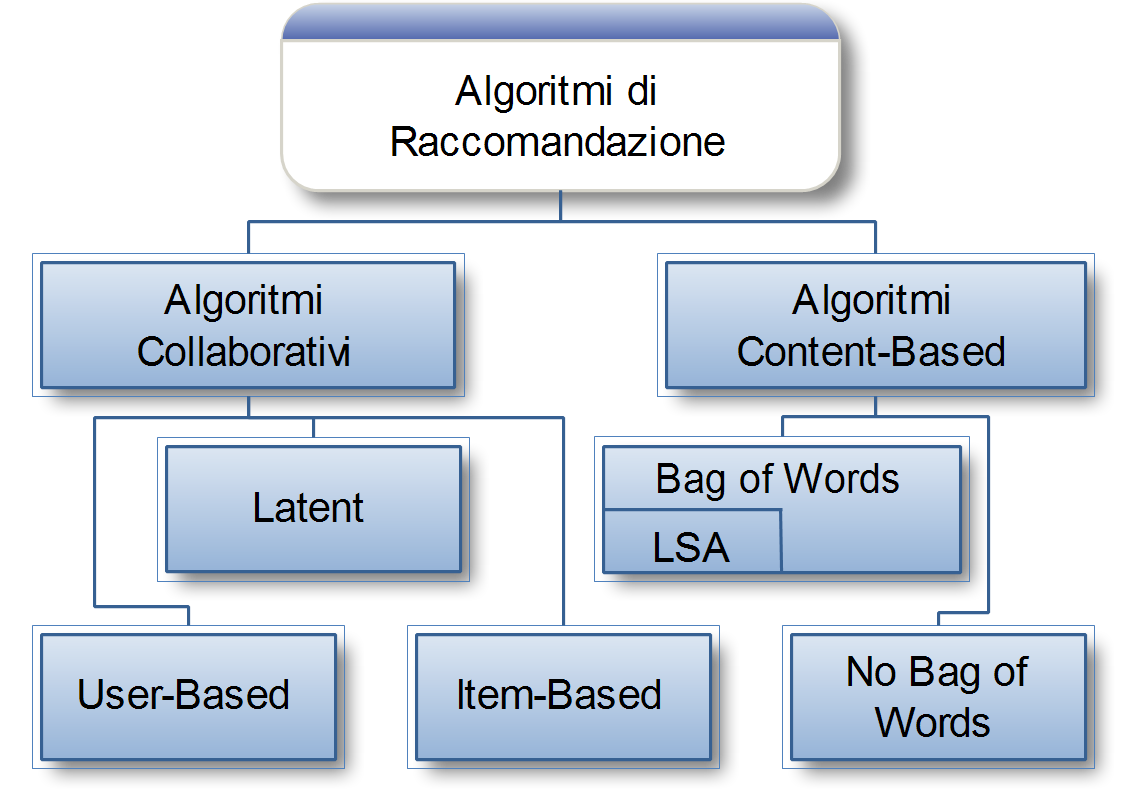
\includegraphics[scale=1]{./img/TipiAlgoritmi}
	\end{center}
	\caption{Classificazione degli algoritmi di Raccomandazione}
	\label{f:algo:algo}
\end{figure}

\subsection{Algoritmi con modello nello spazio latente}
\label{c:algo:algo:lat}

Molto spesso memorizzare tutte le preferenze degli utenti o tutte le caratteristiche di un item � un lavoro che richiede troppo spazio, e di conseguenza anche manipolare questi dati � troppo gravoso dal punto di vista computazionale. Proprio per questo si cerca di diminuire lo spazio utilizzato, avvalendosi del cosiddetto spazio latente. Gli algoritmi che ne fanno uso descrivono il dataset grazie a un insieme ridotto di caratteristiche, dette \corsivo{features}, ricavate attraverso una decomposizione della matrice di partenza. Queste \corsivo{features} possono rappresentare:

\begin{itemize}
	\item l'interazione implicita tra l'utente e l'item nel caso di algoritmi collaborativi (in questo caso si attua una decomposizione della matrice \urm);
	\item il contenuto implicito di ogni item, ovvero gli stem che rappresentano ogni elemento del sistema, nel caso di algoritmi Content-Based (ora invece si ha una decomposizione della matrice \icm).
\end{itemize}

Grazie a questo sistema � anche possibile ridurre notevolmente il rumore generato dall'algoritmo in quanto vengono eliminati i dati meno significativi ai fini della raccomandazione. Una delle tecniche per generare questo spazio latente � la decomposizione matematica SVD (Singolar Value Decomposition). Prende come input la matrice \corsivo{M} di dimensioni $ a \times b $ e la dimensione latente \corsivo{l}, che rappresenta il numero di \corsivo{features} che si vogliono considerare. Il risultato della decomposizione sono tre matrici:

\begin{description}
	\item[U] � una matrice unitaria di dimensioni $ a \times a $;
	\item[S] � una matrice diagonale di dimensioni $ l \times l $ che rappresenta, attraverso valori sempre positivi, le \corsivo{features}, ovvero i valori singolari della matrice \corsivo{M} di partenza;
	\item[V'] � la trasposta coniugata di una matrice unitaria di dimensioni $ b \times b $.
\end{description}

In questo modo quindi si rafforzano i legami tra elementi simili della matrice di partenza, e si riescono anche a trovare dipendenze nascoste tra i diversi elementi.

\subsection{Algoritmi Content-Based}
\label{c:algo:algo:cont}

Si basano sull'analisi delle propriet� dei diversi item, quindi all'utente verranno proposti sempre contenuti simili a quelli che egli stesso ha valutato positivamente. Rappresenta sicuramente il metodo pi� semplice e veloce per effettuare una raccomandazione. Esiste anche un retro della medaglia: dopo aver esaminato tutti i contenuti simili a quelli di suo gradimento, l'utente si ritrover� in sostanza tanti doppioni, o magari, come nel caso dei film, lo stesso elemento, semplicemente rivisitato o reinserito da parte del sistema. Inoltre si possono presentare delle ambiguit�: tornando sempre all'esempio cinematografico, due film possono avere lo stesso regista, un cast simile e per questo essere proposti entrambi, pur essendo di due generi completamente differenti, col rischio che uno dei due non sia di nessun interesse per l'utente.

Per cercare di rimediare a questo inconveniente si pu� restringere l'analisi ad alcuni campi, per esempio non tenere in considerazione il regista, privilegiando altri elementi come il cast. In questo modo si possono proporre contenuti interessanti che l'utente non avrebbe n� pensato n� saputo ricercare. 

Sicuramente si presentano molte problematiche con questo tipo di algoritmi:

\begin{itemize}
	\item Le propriet� degli item devono essere inserite in modo preciso e leggibile dall'algoritmo (poi si vedr� come avviene il ""parsing'' delle stesse).
	\item Le propriet� possono essere sparse: in fase di inserimento sono state ""sottovalutate'' o ignorate talune propriet�, mentre per altri item le stesse sono ritenute molto importanti e specificate. \`E anche possibile che a seconda della persona fisica responsabile dell'inserimento dell'item nel sistema cambino le propriet� scelte: l'operatore \corsivo{A} � molto scrupoloso riguardo al cast, mentre l'operatore \corsivo{B} conosce tutte le sfumature dei generi, per questo introduce anche quelli di nicchia, sconosciuti ai pi�.
	\item Come detto in precedenza due elementi possono avere le stesse propriet�, e magari uno non � di gradimento all'utente: come fa in questo caso l'algoritmo a distinguerli e a capire quale consigliare e quale no?
	\item I suggerimenti sono sempre molto simili agli item gi� visti dall'utente: se ad esempio il fruitore non ha mai visto un film western, il sistema non arriver� mai a consigliargli un film di quel tipo, a discapito di altri che con ogni probabilit� gradirebbe di pi�.
	\item Gli utenti nuovi non riceveranno mai una raccomandazione adeguata in quanto il sistema non ha elementi per fornirgliela, mentre quelli con poche preferenze si vedranno suggeriti pi� volte contenuti identici. Solamente nel caso di profili pi� ""vissuti'' si avranno suggerimenti migliori.
\end{itemize}

La trattazione di questa tipo di algoritmo verter� su quello definito \grassetto{diretto}. Possiamo suddividerlo in diverse fasi, ognuna con la sua funzione specifica:

\begin{description}
	\item[Tokenizzazione] � l'operazione che prende come input le diverse propriet� dell'item e cerca di elaborarne dei token, in modo che possano essere analizzati pi� velocemente. Un token � solitamente una singola parola, ma pu� essere anche una serie di parole come nel caso del nome e del cognome di un attore. Quest'operazione viene effettuata per isolare i termini che in seguito verranno riconosciuti come ""importanti'' per la buona riuscita dell'algoritmo.
	\item[Eliminazione delle Stop Words] avviene subito dopo la suddivisione in token: sono rimossi tutti quegli elementi inutili come ad esempio gli articoli, le congiunzioni e tutte quelle parole che non risultano essere importanti ai fini della raccomandazione.
	\item[Stemmizzazione] modifica parole come sostantivi e aggettivi, eliminando prefissi e suffissi. In questo modo parole simili avranno la stessa valenza per l'algoritmo. Ad esempio le parole ""corsa'', ""correre'' e ""corridore'' saranno tutte riconducibili allo stesso \corsivo{stem} ""cor''. Il risultato di quest'operazione � il cosiddetto \bow (\grassetto{Bag Of Words}).
	\item[Assegnazione di un peso ai metadati] � l'operazione successiva: si effettua un'analisi statistica per calcolare il peso che ogni stem o token ha nei confronti dell'item in cui appare: ad esempio la presenza di un cantante all'interno di un film (magari un cammeo) sar� molto meno importante rispetto alla sua presenza all'interno di un concerto. Si procede quindi al calcolo del TF-IDF (Term Frequency - Inverse Document Frequency). Il Term Frequency � un semplice numero che rappresenta le occorrenze di una parole nelle propriet� di un item. L'Inverse Document Frequency � sempre un numero, l'inverso del numero di occorrenze di un certo token all'interno di tutto il catalogo. Entrambi i pesi possono essere normalizzati per il totale degli elementi del \bow. Da questi pesi se ne ricava uno solo, che viene usato come il valore dell'elemento della matrice \icm.
\end{description}

Si genera quindi uno spazio vettoriale dove gli assi sono i diversi steam che appaiono dentro alla matrice \icm. Gli item vengono rappresentati come vettori in questo spazio. Per completare la raccomandazione si deve disegnare il vettore dell'utente: viene calcolato come la somma dei voti espressi, moltiplicati per la colonna della matrice \icm (quindi per l'item) relativa. Gli item da consigliare saranno poi quelli col coseno dell'angolo compreso tra vettore utente e vettore proprio pi� alto.

\subsubsection{LSA Cosine}
\label{c:algo:algo:cont:lsa}

Questo algoritmo rappresenta lo stato dell'arte per quanto riguarda quelli Content-Based. Si basa su un unico concetto base: l'aggregazione di tutte le parole che compaiono (o non compaiono) all'interno di un testo, stabilisce un insieme di vincoli di reciprocit�, che determinano una similarit� di significato tra le parole stesse, e permette di raggruppare quelle simili. Utilizza, come l'algoritmo Sarwar che tratteremo in seguito, la decomposizione SVD della matrice \icm.

\begin{description}
	\item[Generazione del modello] avviene applicando anzitutto una decomposizione SVD sulla matrice \icm, usando una specifica dimensione latente \corsivo{k}\nota{La definizione del parametro \corsivo{k} � comunemente effettuata in modo empirico.}. Si ottengono quindi tre matrici: $ U_k $, $ S_k $ e $ V_k $. La nuova \corsivo{ICM\pedice{k}}, data dal prodotto $ S_k * V'_k $ e che verr� usata come modello dell'algoritmo, � pulita dal rumore e integra gi� le diverse correlazioni tra gli stem.
	\item[Generazione del suggerimento] ha come input la matrice \urm, il profilo utente e il modello generato in precedenza. Ogni item viene rappresentato nello spazio creato dagli stem del modello. Quindi viene calcolata la similarit� tra il vettore dell'utente e quelli degli elementi che non compaiono nel profilo tramite il coseno dell'angolo compreso tra i due vettori: pi� � alto, pi� l'elemento considerato si avvicina ai gusti dell'utente e quindi il rispettivo contenuto sar� raccomandato.
\end{description}

\subsection{Algoritmi Collaborativi}
\label{c:algo:algo:coll}

A differenza della tipologia vista in precedenza, questi algoritmi si basano solamente sui gusti della comunit� di utenti. Simulano quindi una normale richiesta di suggerimenti tra due esseri umani: se l'utente \corsivo{A} ha un amico con gusti simili, sar� sufficiente chiedergli un consiglio per ritrovarsi con una raccomandazione conforme ai gusti di \corsivo{A}. Si basano su due assunzioni fondamentali:

\begin{description}
	\item[Vicinanza tra utenti] in quanto utenti con gusti simili voteranno sempre gli elementi in maniera simile;
	\item[Vicinanza tra item] poich� gli item ""simili'' saranno votati sempre in maniera simile.
\end{description}

Proprio per questo due contenuti sono valutati simili non tanto quando sono simili tra loro, ma quando la comunit� li vota in modo simile.

A differenza degli algoritmi che si basano sul contenuto, quelli collaborativi possono portare al cosiddetto \grassetto{effetto serendipity} (sorpresa): mentre nel primo caso l'utente comprende sempre il perch� di una raccomandazione, ora pu� rimanere stupito dalla stessa, in quanto gli pu� essere consigliato un elemento fuori dai suoi schemi, ma che � stato votato da soggetti dai gusti simili ai suoi. Proprio qui ha origine uno dei vantaggi maggiori degli algoritmi collaborativi, ovvero il non basarsi su altre informazioni se non i giudizi della comunit�.

Certamente sussistono anche molti limiti a questo tipo di approccio:

\begin{itemize}
	\item quando un nuovo utente entra nel sistema non pu� essere associato a nessun altro utente, quindi non avr� a disposizione una raccomandazione;
	\item all'aggiunta di un nuovo item, esso dovr� essere anzitutto votato da qualcuno in quanto, altrimenti, non verr� associato a nessun item preesistente e quindi non verr� raccomandato;
	\item l'accuratezza della raccomandazione � legata alla sparsit� della matrice \urm: pi� essa � piena di informazioni, pi� sar� preciso il suggerimento;
	\item utenti con gusti particolari saranno associati con molta difficolt� ad altri utenti, e quindi riceveranno suggerimenti poco accurati.
\end{itemize}

All'interno degli algoritmi Collaborativi possiamo effettuare un'ulteriore suddivisione:

\begin{description}
	\item[User-Based] si basano sull'idea di stabilire un rapporto di similitudine tra i diversi utenti della comunit�, in modo da costruire una matrice $ m \times m $ (dove \corsivo{m} � il numero degli utenti). Questi algoritmi hanno problemi per quanto riguarda le performance nella costruzione del modello, in quanto una comunit� pu� avere decine o centinaia di migliaia di utenti iscritti. Un altro tipico problema si ha quando si vuole inserire un nuovo utente: bisogna infatti ricreare completamente il modello, sempre con le problematiche che l'utente nuovo si porta dietro (come visto prima).
	\item[Item-Based] � la tipologia duale di quella precedente: ora si vuole costruire una matrice $ n \times n $ (con \corsivo{n} uguale al numero degli item) che metta in relazione i vari elementi, in modo da trovare quelli simili tra loro. Ogni elemento della matrice � quindi il grado di somiglianza tra l'elemento della riga \corsivo{i} e quello della colonna \corsivo{j} (i numeri sulla diagonale sono ovviamente uguali a 1). Molto spesso questi valori vengono normalizzati, in modo ad averli compresi tra $ -1 $ e $ 1 $ nel caso di rating espliciti, e tra $ 0 $ e $ 1 $ nel caso di rating impliciti. Per eseguire una raccomandazione poi � sufficiente moltiplicare il vettore del profilo utente per la matrice, in modo da ricavare un nuovo vettore con i voti dei singoli item. Una modifica a questo algoritmo � la cosiddetta KNN, in cui la matrice modello viene prima processata ponendo a 0 gli elementi pi� bassi, lasciandone quindi soltanto K. Questo avviene in quanto gli elementi eliminati non influirebbero nella lista finale, ma creerebbero solamente un rumore che quindi andrebbe a risultare fastidioso per la classifica degli altri elementi.
\end{description}

Per quanto riguarda le prestazioni, la creazione del modello negli algoritmi Item-Based sar� pi� rapida in quanto, solitamente, il numero di utenti � di gran lunga superiore a quello di contenuti. Inoltre influisce anche la frequenza con cui un utente o un elemento vengono introdotti nel sistema: anche in questo caso, generalmente, gli utenti nascono con pi� frequenza dei nuovi elementi\nota{Tutte queste ipotesi valgono in condizioni standard: sistemi come YouTube \grassetto{non} sono standard visto che secondo l'ultima stima ogni minuto vengono caricate 35 ore di contenuti audiovisivi.}. Inoltre l'avere un modello Item-Based risulta essere anche comodo quando si aggiunge un nuovo elemento al sistema: dal momento che questo, prima di essere raccomandato, dovr� raccogliere un certo numero di voti, non � necessario che il modello venga ricreato istantaneamente, quindi non c'� la frenesia che ci sarebbe per il modello User-Based dove ad ogni aggiunta bisogna assolutamente creare un nuovo modello.

\subsubsection{Item-Item Cosine KNN}
\label{c:algo:algo:coll:iic}

Rientra nella categoria degli algoritmi Item-Based. Ogni elemento del sistema � visto come un vettore nello spazio degli utenti: la similitudine tra due vettori � rappresentata come il coseno dell'angolo tra essi compreso:

\begin{equation}
\label{e:algo:iic:sim}
	sim(i, j) = cos(\vec{i}, \vec{j}) = \frac{\vec{i} \cdot \vec{j}}{\|\vec{i}\|^2 \times \|\vec{j}\|^2}
\end{equation}

Questo coefficiente sar� uguale a 1 nel caso in cui due elementi siano uguali, e a 0 nel caso due elementi non abbiano voti in comune.

Nella fase di raccomandazione, invece, il calcolo da effettuare sar� molto pi� semplice: 

\begin{equation}
\label{e:algo:iic:rac}
	Raccomandazione = Profilo Utente \cdot Modello
\end{equation}

Questa sar� una lista di voti: nel caso di dataset esplicito si avr� la predizione del voto che l'utente avrebbe dato a quello specifico elemento, mentre nel caso di un dataset implicito sar� la probabilit� con cui l'utente potrebbe aver visto quel contenuto ma non aver dato una votazione. In seguito il sistema ordiner� questi voti in ordine decrescente e ne estrarr� i primi N, generando quindi la tanto attesa Top-N da suggerire all'utente stesso.

Il parametro KNN (\corsivo{K Nearest Neighbor}) indica il numero di elementi da tenere in considerazione in fase di creazione del modello, quando vengono trovati i coefficienti di similarit� tra i diversi item. Si vanno infatti a utilizzare solamente i K elementi pi� vicini a quello in fase di analisi. L'eliminazione di tutti gli altri elementi si basa sulla convinzione che essi generino solamente rumore. Questo parametro ha il suo fondamento nella dimensione del dataset: pi� � piccolo pi� sar� precisa la raccomandazione, ma un parametro troppo piccolo rispetto alla matrice potrebbe eliminare troppo rumore, e quindi danneggiare la raccomandazione stessa che andrebbe a consigliare solamente elementi troppo vicini a quelli di partenza. Quando K tende a infinito, l'algoritmo perde la sua propriet� KNN e si definisce solamente Item-Item Cosine.

\subsubsection{Item-Item DR}
\label{c:algo:algo:coll:iidr}

Questo algoritmo (dove DR sta per Direct Relation) � simile al precedente. L'unica differenza � che la similarit� tra due elementi della matrice viene calcolata come il numero di occorrenze in cui entrambi gli item sono presenti tra tutti i profili utenti. La fase di raccomandazione, poi, � sempre una semplice moltiplicazione tra il vettore utente e la matrice del modello.

\subsubsection{Sarwar}
\label{c:algo:algo:coll:sar}

Sempre della famiglia degli Item-Based, questo algoritmo utilizza la decomposizione SVD sulla matrice \urm per ridurre lo spazio fisico occupato. Infatti si utilizzer� solamente una delle tre matrici calcolate tramite la decomposizione. La matrice di similarit� tra elementi viene calcolata con i seguenti passaggi:

\begin{enumerate}
	\item si riceve come input la matrice \urm e un parametro \corsivo{ls} che rappresenta la dimensione dello spazio latente in cui costruire la matrice modello;
	\item si applica la decomposizione SVD alla matrice \urm ($ m \times n $), utilizzando lo spazio latente \corsivo{ls}: si ottengono quindi le matrici $ U $ ($ m \times ls $), $ S $ ($ ls \times ls $), $ V' $ ($ ls \times n $). Quest'ultima matrice $ V' $ rappresenta il modello dell'algoritmo e, come si pu� facilmente verificare, � di dimensioni minori rispetto a tutte quelle $ n \times n $ utilizzate in precedenza;
	\item si moltiplica $ V \times V' $ in modo da ottenere la matrice di similarit� (il modello vero e proprio): questa viene creata solamente per i calcoli, in quanto per la memorizzazione si utilizza sempre solo $ V' $.
\end{enumerate}

Infine per ottenere la raccomandazione si effettua sempre la solita moltiplicazione del vettore del profilo utente per la matrice di similarit�, ottenendo un coefficiente per ogni elemento. Ordinando poi in ordine decrescente i coefficienti si avr� la lista Top-N da suggerire.

\subsubsection{Asymmetric SVD}
\label{c:algo:algo:coll:kor}

Ideato da Yehuda Koren, questo algoritmo\cite{Koren} Item-Based � stato il vincitore della competizione Netflix Prize, e quindi si � imposto come lo stato dell'arte per quanto riguarda gli algoritmi collaborativi. \`E in grado di lavorare sia con dataset impliciti sia espliciti.

Per ogni elemento \corsivo{i} non presente nel profilo dell'utente \corsivo{u} viene calcolato un rating per mezzo della seguente formula:

\begin{equation}
\label{e:algo:kor:rat}
	r_{ui} = b_{ui} + q^T_i(|R(u)|^{-{1 \over 2}} \sum_{j \in R(u)} (r_{uj} - b_{uj}) x_{j} + (|N(u)|)^{-{1 \over 2}} \sum_{j \in N(u)} y_{j})
\end{equation}

Analizziamo ora nel dettaglio la formula:
\begin{description}
	\item[$ b_{ui} = \mu + b_{u} + b_{i} $] dove $ \mu $ � la media dei rating del dataset, mentre $ b_{u} $ e $ b_{i} $ sono le distanze (\corsivo{bias}) rispettivamente dei ratings dell'utente $ u $ e della media dei ratings ricevuti dall'item $ i $ rispetto alla media totale $ \mu $;
	\item[$ |R(u)| $] � la cardinalit� dell'insieme dei ratings \corsivo{espliciti} dell'utente $ u $;
	\item[$ |N(u)| $] � la cardinalit� dell'insieme dei ratings \corsivo{impliciti} dell'utente $ u $;
	\item[$ q $] � il vettore degli elementi $ i $ non votati dall'utente;
	\item[$ x $] � il vettore degli elementi $ j $ che hanno ricevuto un rating esplicito;
	\item[$ y $] � il vettore degli elementi $ j $ che hanno ricevuto un rating implicito.
\end{description}

Questo algoritmo � stato poi leggermente modificato per adattarlo anche a scenari differenti da quello del Netflix Prize:

\begin{itemize}
	\item alcuni parametri che intervenivano durante la creazione del modello sono stati cambiati in quanto si verificava overfitting sul bias degli utenti e degli elementi, portando quindi la raccomandazione ad essere sempre identica;
	\item durante la raccomandazione si verifica un ulteriore apprendimento sul profilo dell'utente: per questo � stata leggermente modificata questa fase per poter utilizzare anche dei profili creati ad hoc e non necessariamente facenti parte della matrice \urm.
\end{itemize}
\chapter{Metodologie di Test}
\label{c:met}

Lo studio dei sistemi di raccomandazione dipende in grandissima parte dalla buona qualit� dei risultati che si ottengono: il fine ultimo, infatti, � quello di fornire suggerimenti all'utente per invogliarlo ad acquistare contenuti multimediali. Se i suggerimenti risultano essere adeguati e quindi l'utente d� fiducia al sistema , si incrementeranno sia gli acquisti sia la soddisfazione generale. Se invece l'utente si accorge che le raccomandazioni fornite non risultano essere attendibili, si creer� un'insoddisfazione nei confronti del sistema, e di conseguenza diminuir� il numero degli acquisti.

Ma come si fa a capire se un algoritmo raccomanda elementi in modo adeguato o meno? In questa circostanza viene in aiuto la statistica, mostrando delle metodologie di test che generano un metro di giudizio per ogni singolo test.

\section{Hold Out}
\label{c:met:ho}

\begin{figure}
	\begin{center}
		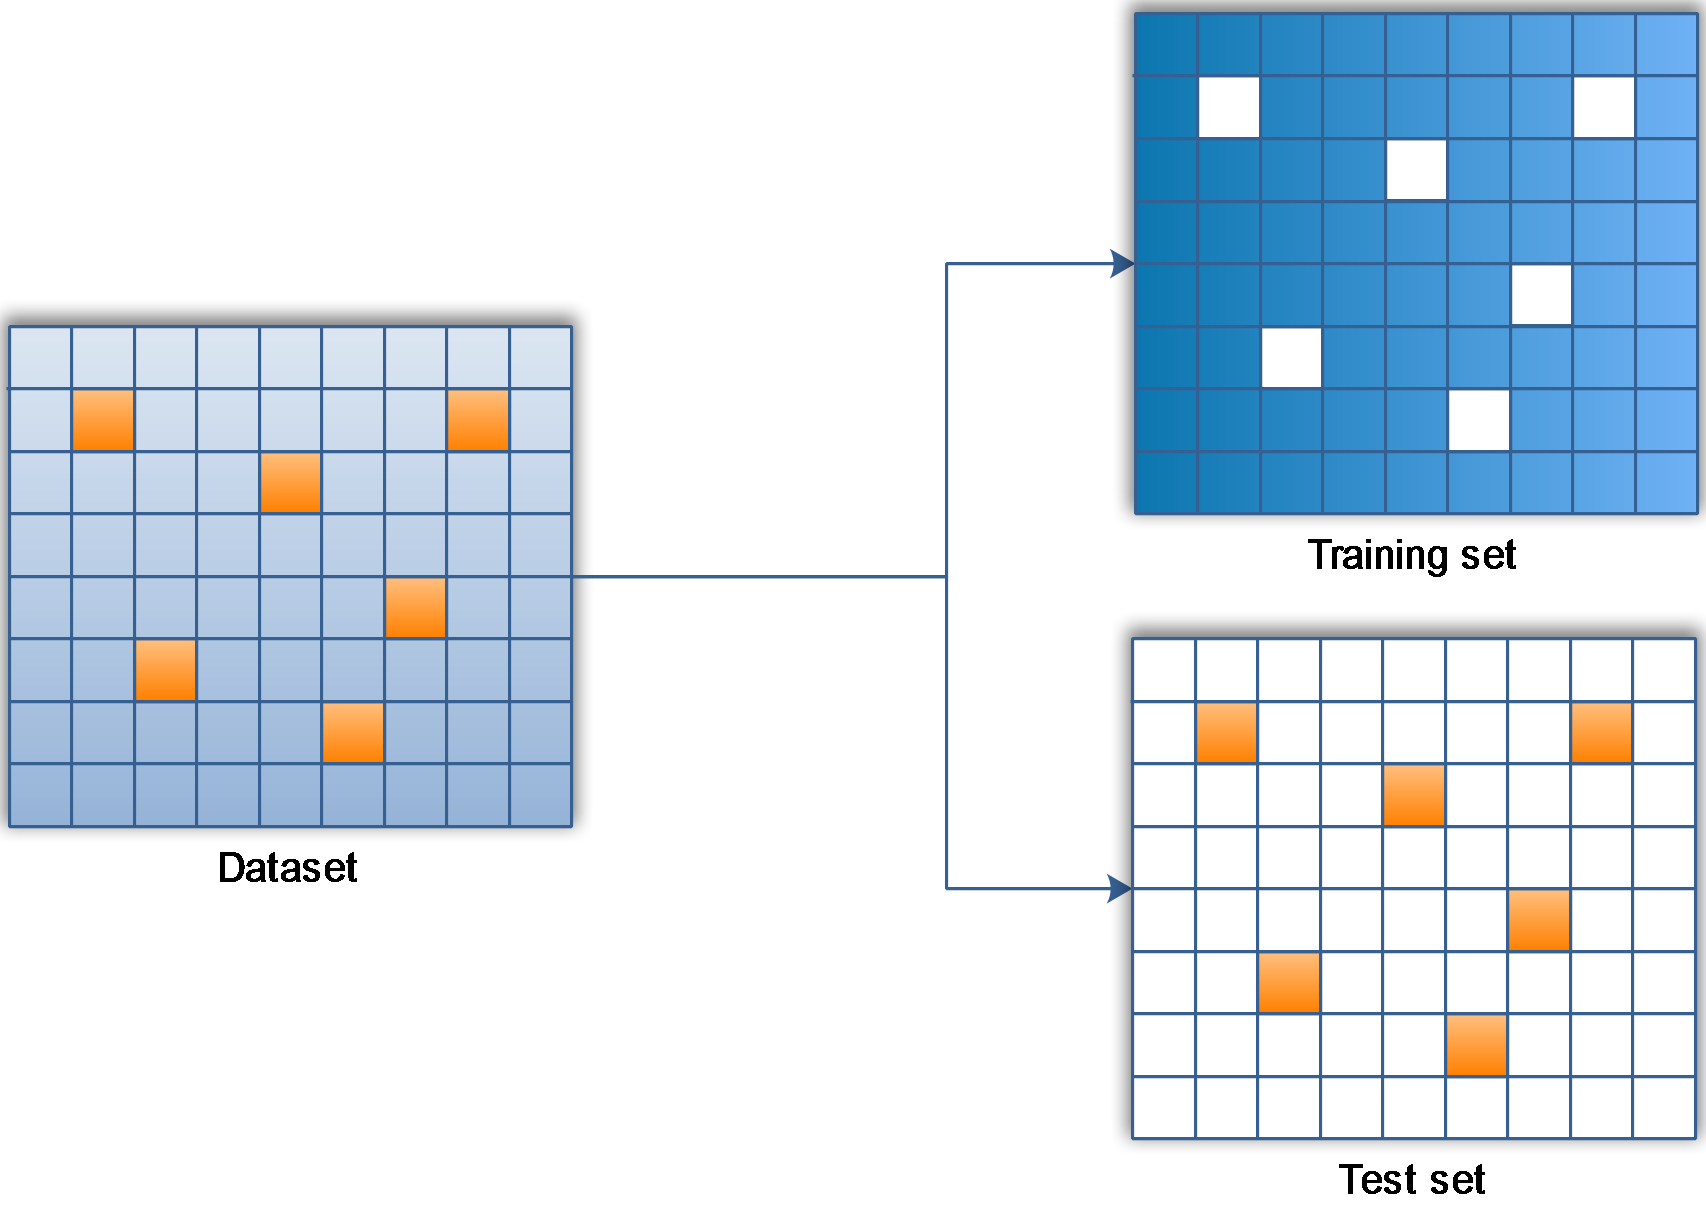
\includegraphics[scale=1]{./img/HoldOut}
	\end{center}
	\caption{Metodologia HoldOut}
	\label{f:met:ho}
\end{figure}

La pi� semplice in assoluto forma di test si ottiene prendendo una piccola percentuale del dataset (solitamente intorno al 3\%) e facendola diventare il TestSet. La restante parte forma invece il TrainSet. Com'� facilmente intuibile in fase di testing si usa il TrainSet per creare il modello che verr� usato in seguito per stimare i risultati del TestSet.

Questo test ha il vantaggio di essere il pi� semplice di tutti, ma si dimostra anche molto inefficiente in quanto all'interno della percentuale usata come TestSet si possono presentare eccezioni o casi particolari. Un rimedio a ci� pu� essere fornito dall'introduzione di filtri\nota{Si pu� ad esempio decidere di prendere in considerazione solamente i voti superiori una certa soglia nel caso di dataset espliciti, oppure utenti che han fornito almeno un certo numero di preferenze.} durante la suddivisione del dataset, ma anche questo non sempre risolve i problemi. Ci si affida quindi ad altre metodologie per ottenere risultati pi� accurati, mentre questa viene utilizzata se si vuole una stima rapida (seppur imprecisa) del tutto, visto che gli altri metodi sono incredibilmente pi� complessi dal punto di vista computazionale.

\section{K-Fold Cross Validation}
\label{c:met:kf}

\begin{figure}
	\begin{center}
		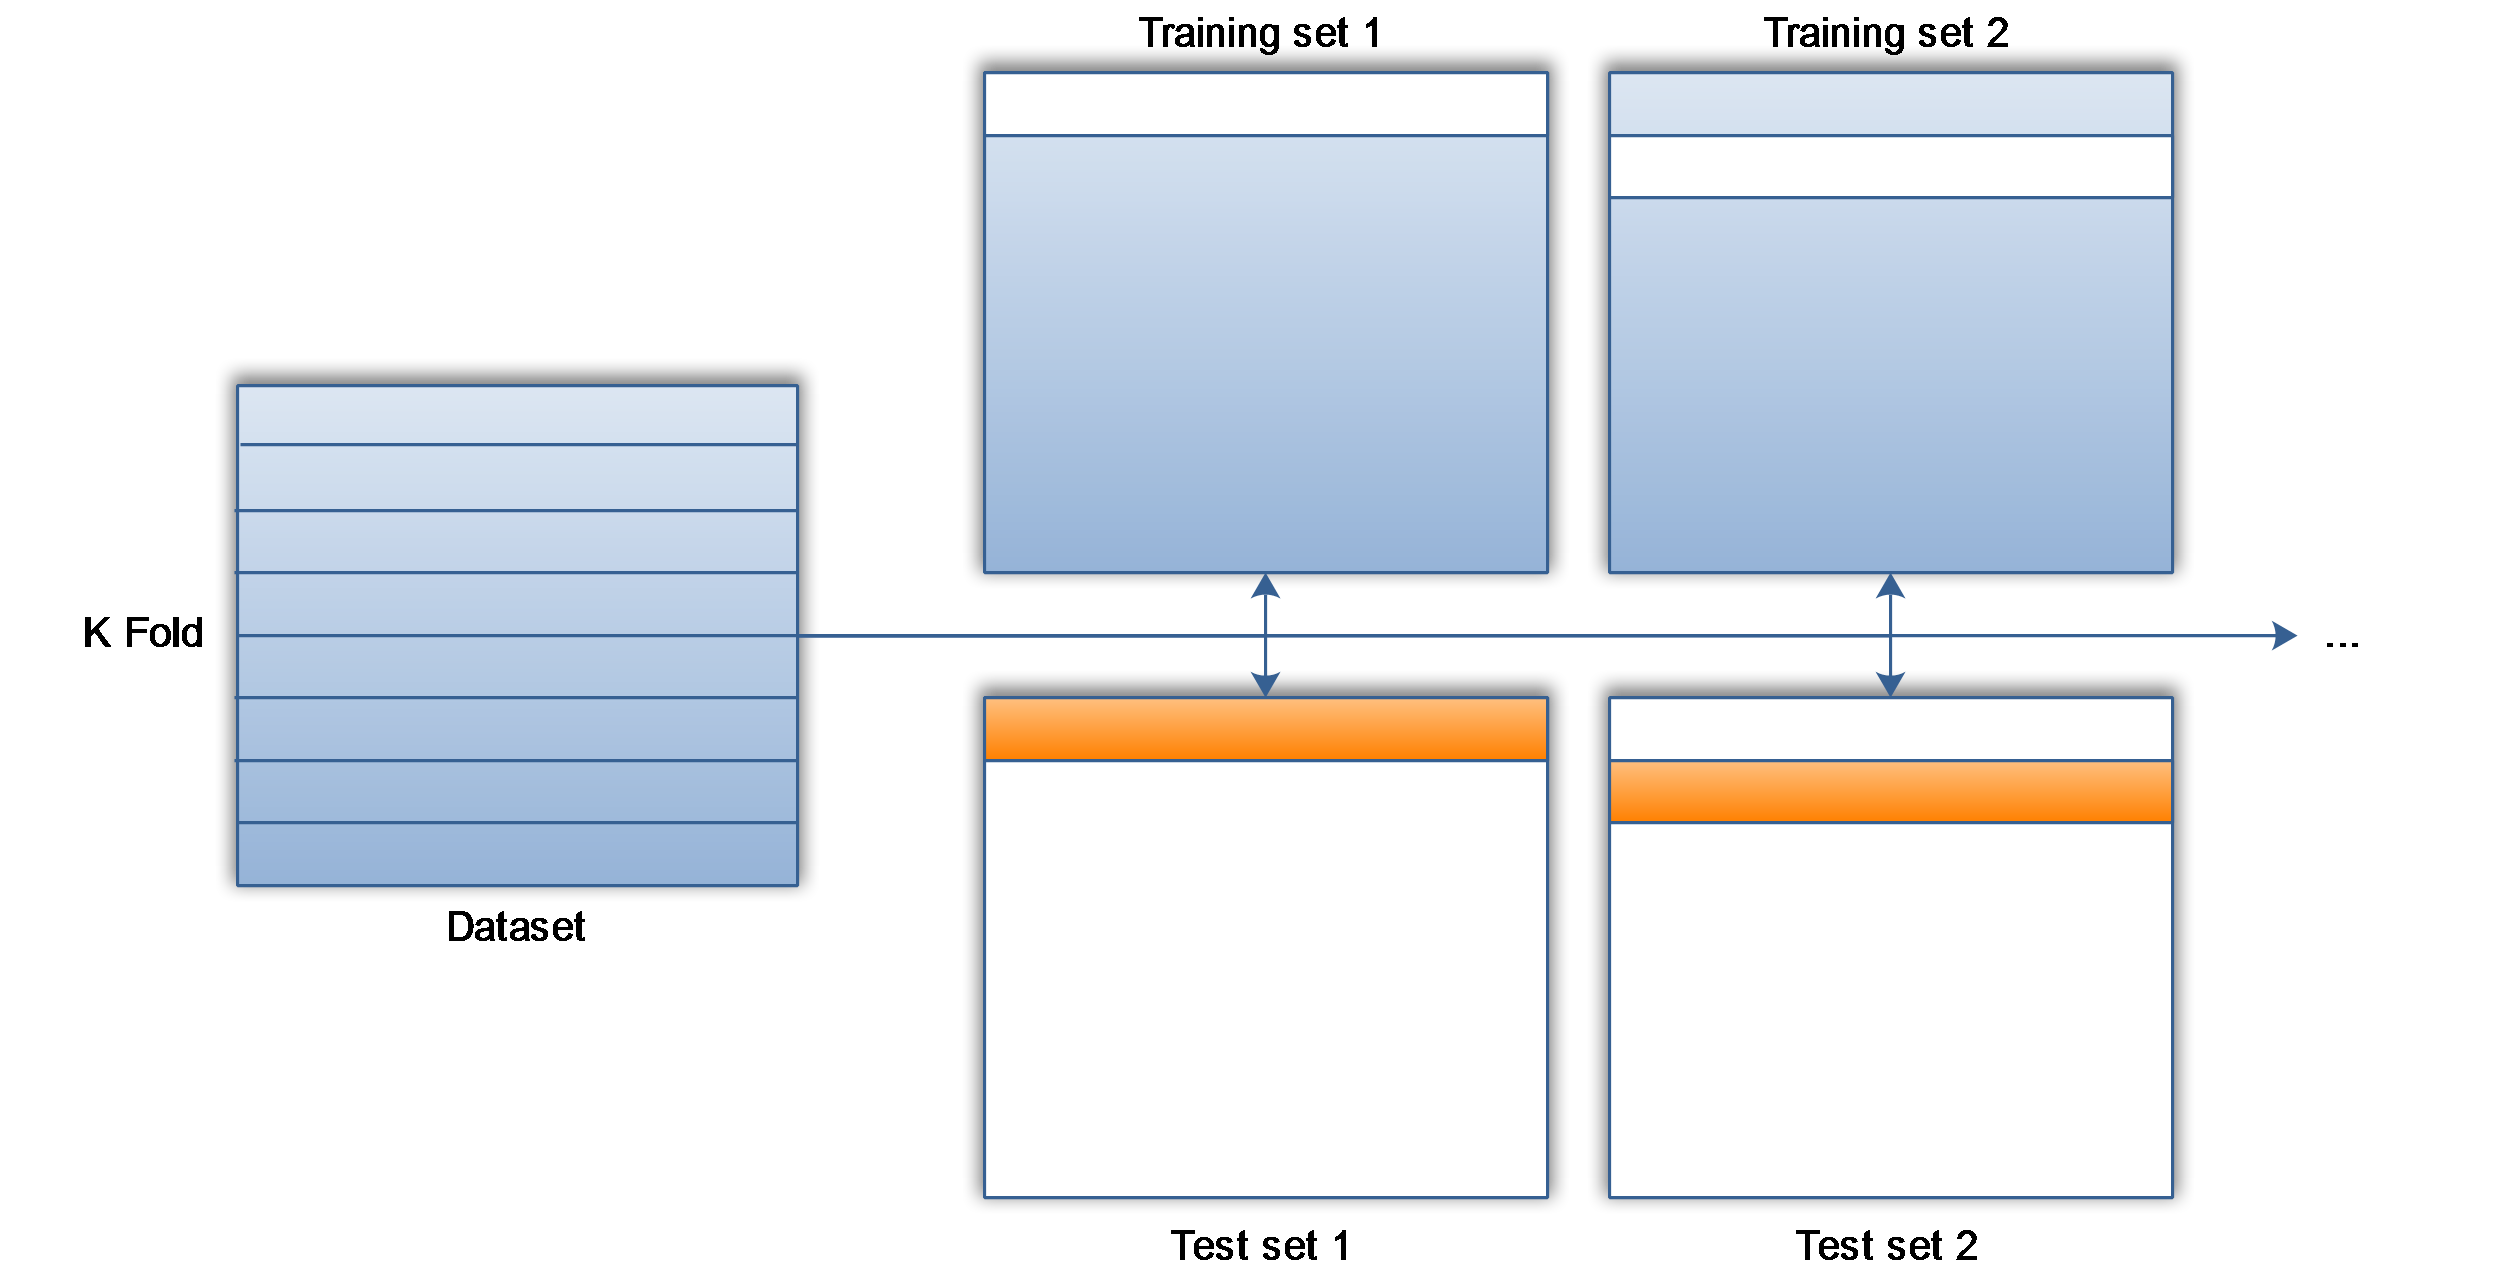
\includegraphics[scale=0.7]{./img/KFold}
	\end{center}
	\caption{Metodologia K-Fold Cross Validation}
	\label{f:met:kf}
\end{figure}

Questa tipologia di test consiste nello stimare l'affidabilit� di un'analisi in base a un campione indipendente. Il dataset viene suddiviso casualmente in \corsivo{K} parti con la stessa cardinalit�. Una alla volta queste parti diventano il campione di validazione, mentre le restanti $ K - 1 $ sono il campione di training. Questo procedimento viene ripetuto $ K $ volte in modo che tutte le parti diventino, una alla volta, campione di validazione. Durante la validazione di una parte, le altre servono per il training, quindi per la creazione del modello. Questa validazione viene realizzata analizzando un singolo campione del TestSet alla volta, con un meccanismo chiamato Leave One Out (analizzato in seguito): in questo caso per� il modello � gi� stato creato e si usa sempre quello.

I risultati ottenuti dopo tutti i campionamenti vengono riuniti per generare un unico risultato che fornisca la stima cercata. Il vantaggio di questo metodo � quindi che ogni parte del dataset faccia da validazione e da training, in modo da non generare overfitting. In letteratura a \corsivo{K} viene solitamente attribuito il valore 10.

\section{Leave One Out Cross Validation}
\label{c:met:loo}

\begin{figure}
	\begin{center}
		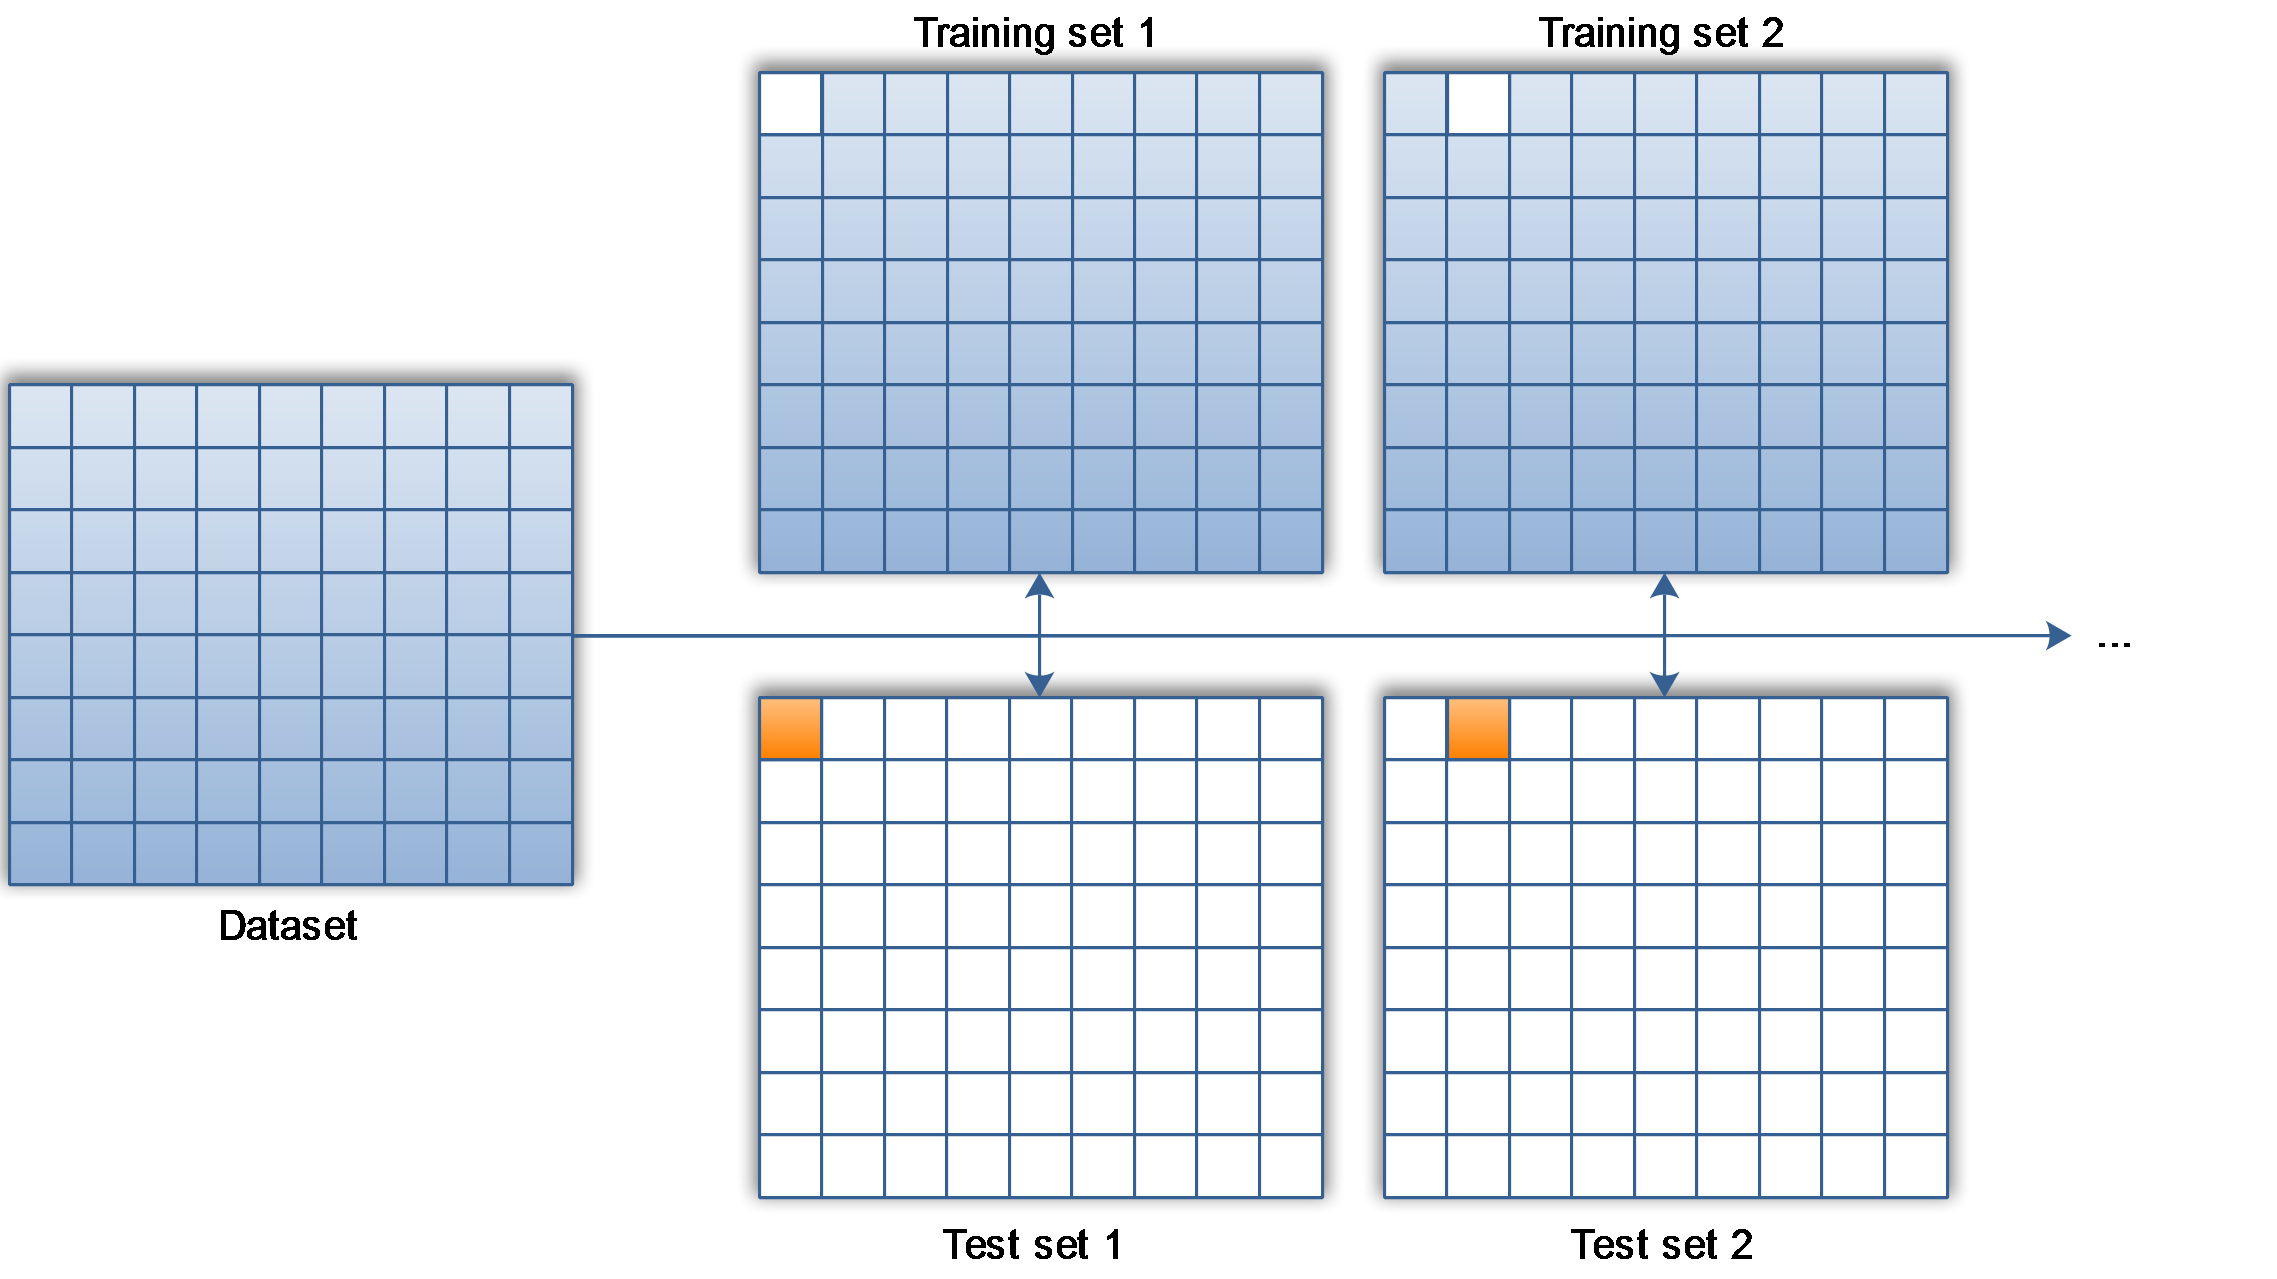
\includegraphics[scale=0.7]{./img/LeaveOneOut}
	\end{center}
	\caption{Metodologia Leave One Out}
	\label{f:met:loo}
\end{figure}

Un caso particolare del metodo esaminato prima � il Leave One Out, dove in pratica si assegna a \corsivo{K} il valore della cardinalit� del dataset. Viene testato un solo valore alla volta, usando tutti gli altri per il training.

Questa validazione pu� essere considerata migliore di quella precedente in quanto si riesce a indicare con pi� precisione se esistono dei casi per cui l'algoritmo sbaglia, fornendo raccomandazioni errate. C'� anche da dire, per�, che computazionalmente � molto pi� pesante in quanto il modello deve essere ricreato molte pi� volte rispetto al semplice K-Fold, quindi si cerca di usarlo solamente per problemi di piccole dimensioni.

\section{Metriche}
\label{c:met:met}

Dopo aver esaminato le varie tipologie di test si passa ora a capire esattamente come si pu� valutare un algoritmo e quali metri di giudizio si hanno per determinare se conviene o meno.

Si usano quindi delle metriche, valori che mostrano (su una scala relativa o assoluta) un giudizio su quanto � stato valutato dal test, in modo da riuscire a classificare in modo semplice e rapido i vari algoritmi. In seguito verranno mostrate le varie metriche, suddividendole in:

\begin{itemize}
	\item Metriche di errore;
	\item Metriche di classificazione.
\end{itemize}

\subsection{Metriche di errore}
\label{c:met:met:err}

Servono normalmente per valutare la predizione di un rating\nota{Il campo normale di utilizzo sono i rating espliciti in quanto viene valutata la distanza tra la predizione e il valore vero. Possono essere anche utilizzate in presenza di valutazioni implicite, ma in questo modo non riescono ad avere tutta la potenza di espressione che hanno nel caso di rating espliciti.}. Non sono molto utilizzate in quanto gli algoritmi correttivi influiscono solamente sulla posizione nella classifica ritornata dalla fase di raccomandazione, e non sulla valutazione stessa.

\subsubsection{Mean Absolute Error (MAE)}
\label{c:met:met:err:mae}

Letteralmente � l'\corsivo{Errore Medio Assoluto} e rappresenta la distanza media tra il valore predetto e quello reale. Questa distanza �, ovviamente, calcolata in valore assoluto:

\begin{equation}
\label{e:met:mae}
	MAE = {1 \over n} \sum_{i = 1}^{n} |\hat{r}_{ij} - r_{ij}|
\end{equation}

\subsubsection{Mean Squared Error (MSE)}
\label{c:met:met:err:mse}

Viene tradotto letteralmente come \corsivo{Errore Quadratico Medio} ed � la differenza quadratica media tra i valori osservati e i valori attesi. Si calcola in modo simile al MAE:

\begin{equation}
\label{e:met:mse}
	MSE = {1 \over n} \sum_{i = 1}^{n} {(\hat{r}_{ij} - r_{ij})}^2
\end{equation}

\subsubsection{Root Mean Squared Error (RMSE)}
\label{c:met:met:err:rmse}

\`E la radice quadrata dell'MSE e rappresenta la varianza interna data dal rapporto fra la devianza interna e la numerosit� totale:

\begin{equation}
\label{e:met:rmse}
	RMSE = \sqrt{MSE}
\end{equation}

\subsection{Metriche di classificazione}
\label{c:met:met:clas}

\subsubsection{Recall}
\label{c:met:met:class:rec}

Nella raccomandazione, un elemento pu� essere fondamentalmente di due tipi: rilevante per l'utente, che quindi si aspetta di trovarlo in cima alla lista, con un punteggio alto, oppure non rilevante per l'utente, che quindi si stupirebbe se fosse nella parte alta della lista. Proprio per questi motivi ogni elemento raccomandato pu� essere classificato in uno dei seguenti modi:

\begin{description}
	\item[True Positive (TP)] item consigliati dal sistema e rilevanti per l'utente, ovvero quelli che giustamente ricoprono una posizione alta nella classifica;
	\item[False Positive (FP)] item consigliati dal sistema, ma che non ricoprono un ruolo rilevante per l'utente; rappresentano gli errori ""positivi'' del sistema;
	\item[True Negative (TN)] elementi che non sono consigliati dal sistema e che non sono rilevanti per l'utente, quindi quelli che giustamente hanno un rating basso;
	\item[False Negative (FN)] elementi che non vengono raccomandati dal sistema, ma che l'utente vorrebbe vedersi consigliati.
\end{description}

La recall, una delle metriche pi� accurate per valutare le prestazioni di un algoritmo di raccomandazione, si basa su un'idea molto semplice: quanti elementi rilevanti sono stati consigliati tra tutti quelli interessanti per l'utente? In formule:

\begin{equation}
\label{e:met:rec}
	Recall = {TP \over {TP + FN}}
\end{equation}

Proprio per questa sua caratteristica di considerare una percentuale del totale degli elementi viene definita una metrica di completezza che dipende molto dalla lunghezza della lista da raccomandare, quindi dal parametro N della lista Top-N: per ""positivi'' e ""negativi'' infatti si intendono quegli elementi che compaiono o meno nelle prime N posizioni della lista.

Com'� ovvio pensare, a valori alti di recall corrispondono algoritmi pi� accurati\nota{Il valore massimo della recall sar� 1 quando non esistono ""false negative'', mentre sar� 0 nel caso pessimo, ovvero quando non esistono ""true positive''.}.

\subsubsection{Precision}
\label{c:met:met:class:pre}

Anche questa � una delle metriche pi� accurate nella valutazione di un algoritmo di raccomandazione, ma, a differenza della recall, non misura la completezza, bens� l'esattezza e l'affidabilit� dell'algoritmo, misurando infatti la percentuale di elementi consigliati che l'utente trova rilevanti, rispetto al numero di quelli raccomandati in totale\nota{Nella formula seguente \corsivo{N} � lo stesso di \corsivo{Top-N}, rappresenta quindi il numero di elementi che rientrano nella raccomandazione visibile all'utente.}:

\begin{equation}
\label{e:met:pre}
	Precision = {TP \over N}
\end{equation}

Come si � visto per la recall, anche questa metrica dipende fortemente dal parametro N.

\subsubsection{Expect Percentile Ranking (EPR)}
\label{c:met:met:class:epr}

La \corsivo{Votazione Attesa Percentuale} � una misura della qualit� che considera altro oltre alla lista Top-N: preso infatti un campione di raccomandazioni indica, percentualmente, la posizione in classifica in cui vengono consigliati gli elementi. Si calcola nel seguente modo:

\begin{equation}
\label{e:met:epr}
	EPR = {{\sum_{u, i} r^T_u i \times rank_u i} \over {\sum_{u, i} r^T_u i}}
\end{equation}

\`E quindi la somma delle posizioni in classifica di tutti gli item del campione preso in esame, diviso per la sua numerosit�.

Pi� � basso il valore dell'EPR, pi� il sistema ha predetto gli elementi visti dall'utente nelle prime posizioni. Il 50\% corrisponde a una raccomandazione effettuata prendendo i valori in modo casuale, e pi� si cresce pi� lo scenario peggiora.

\subsubsection{Average Reciprocal Hit Rank (ARHR)}
\label{c:met:met:class:arhr}

\`E una misura della qualit� che esamina la posizione in cui un elemento viene raccomandato all'interno della lista stessa. Si ripensi alla precision e la si ridefinisca come il rapporto tra una raccomandazione ritenuta importante per l'utente (ovvero un TP), chiamata \corsivo{hit} e il numero \corsivo{n} di raccomandazioni:

\begin{equation}
\label{e:met:hr}
	HitRate = {\#Hits \over n}
\end{equation}

Quando l'Hit Rate � uguale a 1, l'algoritmo � riuscito a raccomandare tutti gli elementi rilevanti. Non viene per� presa in considerazione la posizione in classifica in cui viene consigliato l'elemento: non c'� differenza se quello meno rilevante � stato suggerito per primo mentre quello pi� rilevante compare all'ultimo posto.

Superiamo questa limitazione utilizzando la metrica ARHR che d� un punteggio a ogni hit, sulla base della posizione nella lista. Definito \corsivo{h} il numero di hit che avvengono nelle posizioni \corsivo{p\pedice{1}}, \corsivo{p\pedice{2}}, \dots, \corsivo{p\pedice{N}}: 

\begin{equation}
\label{e:met:arhr}
	ARHR = {1 \over n} \sum_{i = 1}^{h} {1 \over {p_i}}
\end{equation}

Agendo in questo modo gli hit nelle posizioni alte della classifica valgono di pi� di quelli nelle posizioni basse. Se gli elementi compaiono tutti in prima posizione, allora il valore dell'ARHR coincide con quello dell'Hit Rate. Quando invece gli hit avvengono nelle posizioni basse della classifica l'ARHR diminuisce fino ad arrivare al valore limite di $ {{HR} \over n} $.
\chapter{Analisi dell'applicazione e descrizione del problema}
\label{c:stato}

La trattazione va ora a prendere in esame la piattaforma di raccomandazione com'era prima di questo lavoro di tesi, esaminandone attentamente i difetti che poi hanno portato alla volont� di ripartire da zero per costruire una piattaforma pi� dinamica e agile.

\section{La partenza}
\label{c:stato:part}

Alla creazione della piattaforma certo non si pensava che risultasse qualcosa di cos� complesso: si sentiva solamente la necessit� di implementare qualche algoritmo di raccomandazione, pi� per esercizio che per altro: non si era presa in esame una possibile integrazione dei vari algoritmi, per questo furono creati completamente diversi gli uni con gli altri\nota{Come esempio basti citare il nome del parametro con cui veniva passato il modello gi� creato: in ogni algoritmo che implementa questa possibilit�, nemmeno in tutti, si usa un nome diverso che riflette le caratteristiche del determinato modello.} e ognuno con i suoi parametri.

Procedendo col lavoro si evidenziarono i limiti di queste strutture, e soprattutto i limiti di MatLab che seppur semplificando molte operazioni, non riesce a raggiungere le velocit� tipiche del C e di altri linguaggi di programmazione pi� a basso livello. Fu cos� che le funzioni pi� impegnative vennero implementate in C, riuscendo a garantire per lo meno standard prestazionali di gran lunga superiori a quelli precedenti.

Continuava a rimanere, per�, sempre un qualcosa di slegato e fine a se stesso, lontano dal suscitare il ben che minimo interesse.

\section{NetFlix e i test}
\label{c:stato:nf}

Finalmente arriv� dall'esterno una spinta per iniziare a dare un senso a tutti gli algoritmi inseriti e funzionanti: un provider di \iptv statunitense indisse una competizione per trovare l'algoritmo di raccomandazione migliore al mondo. Da tutte le migliori universit� e centri di ricerca iniziarono ad arrivare tonnellate di algoritmi che vennero processati da NetFlix\cite{Netflix} stesso per verificarne la bont�.

Alla fine vinse la competizione Yehuda Koren col suo algoritmo ""Asymmetric SVD'' (cfr. \ref{c:algo:algo:coll:kor}), ma il sistema in oggetto di questo lavoro di tesi inizi� a implementare tutte quelle metodologie di test che hanno permesso a NetFlix di valutare i vari lavori.

Nacque cos� l'idea di organizzare i vari algoritmi, che comunque erano ancora disuniti e privi di un filo conduttore che ne guidasse l'implementazione, per lo meno in directory e nel numero di input. Cos� facendo ogni metodo di test poteva utilizzare qualsiasi algoritmo per creare il modello e quindi la raccomandazione da valutare.

Contemporaneamente all'implementazione dei test si cerc� anche si sistemare gli algoritmi gi� visti per poterli migliorare e adattare alla nuova piattaforma: vennero infatti creati degli studi per sistemare alcuni algoritmi particolarmente complessi, in modo da semplificarli e renderli pi� adatti alla piattaforma che ormai era stata prodotta, seppur ancora adatta solamente a chi ci lavora quotidianamente.

\section{Le novit�}
\label{c:stato:news}

Iniziarono finalmente ad arrivare anche le prime novit� apportate alla piattaforma: prima fra tutte l'antireshuffling (cfr. \ref{c:algo:compo}) che introduceva una logica nuova nella creazione delle liste di raccomandazione.

Quest'aggiunta, per�, veniva implementata scontrandosi contro la frammentariet� dell'opera fino ad allora prodotta, quindi era stata creata una struttura incredibilmente fragile di funzioni che necessitavano di parametri incredibilmente specifici per funzionare: utilizzare queste funzionalit� risultava praticamente impossibile se prima non si veniva sottoposti a una sessione di training.

Man mano furono anche aggiunte una serie di metodologie di test differenti, prese in letteratura e implementate in modo sommario, al solo fine di ottenere determinati risultati ma senza la necessit� di legare le varie strutture di dati o i risultati stessi.

\section{Lo stop}
\label{c:stato:stop}

Era questo il momento giusto per fermarsi e riflettere: per quanto tempo poteva ancora essere interessante una struttura del genere, completamente frammentata e in cui ogni riga di codice era fine a se stessa? Quanto poteva servire una piattaforma simile, dove comparivano tanti risultati che se considerati contemporaneamente risultavano inutili in quanto slegati?

Si decise quindi di fermare, almeno in parte, la ricerca e focalizzare l'attenzione sul rifacimento dell'intero sistema, in maniera pi� intuitiva e soprattutto avendo sott'occhio l'intero lavoro: non si pensava pi� di dover solamente costruire alcuni algoritmi come esercizio, ma c'era la necessit� di permettere la scalabilit� della struttura, la facile integrazione di nuovi algoritmi che potessero essere presi facilmente dal sistema e utilizzati attraverso semplici API.

Anche le metodologie di test dovevano essere raccolte e adattate al sistema, in modo che ne risultassero facili sia l'ampliamento sia la modifica.

Ormai si era arrivati al punto di impiegare pi� tempo per comprendere la piattaforma che per implementare nuove funzionalit� o studiarne i risultati.

\section{Altri esempi esterni a questo progetto}
\label{c:stato:altri}

Per cercare di capire meglio come organizzare il lavoro e soprattutto su quali aspetti agire, si � guardato anche ad altri progetti realizzati in altre parti del mondo. Tra tutti quelli trovati, si � deciso di citarne solamente alcuni in quanto costituiscono un campione esemplare.

\subsection{Open Source Recommender System Software Workshop}
\label{c:stato:altri:work}

Viene inserito questo progetto\cite{OSWorkshop} per primo in quanto costituisce il miglior tentativo (anche se poi si � rivelato il peggiore visto che � stato cancellato quasi subito) di realizzare una piattaforma opensource dedicata ai sistemi di raccomandazione.

L'idea di fondo degli sviluppatori che ebbero l'idea era creare una comunit� di studenti e professionisti intorno a questa piattaforma, in modo da non dipendere sempre da quanto sviluppato dalle aziende: la loro idea era che le soluzioni a pagamento fossero troppo poco trasparenti, e quindi si rivelassero alla lunga non interessanti da un punto di vista puramente didattico. 

Proprio per questo si volle creare un progetto aperto a tutti con la speranza che, grazie al web e alla disponibilit� degli utenti, si riuscisse a dare alla luce una valida alternativa alle piattaforme proprietarie, rendendo i sistemi di raccomandazione un qualcosa di pi� facilmente capibile e utilizzabile. Inoltre una soluzione del genere poteva essere accolta positivamente anche dagli sviluppatori e dalle aziende del settore, che l'avrebbero presa come base da ampliare: fa sempre comodo avere delle fondamenta comode e indipendenti per svilupparci sopra le proprie idee.

Sfortunatamente tutti questi buoni propositi non ebbero seguito in quanto la prima conferenza sull'argomento venne cancellata in quanto non vi erano iscritti, e dopo poco tempo, anche l'intero progetto mor� dal momento che la comunit� sognata non si era creata. A un anno dalla data della conferenza, l'unica traccia che rimane di questo lavoro � il \grassetto{Duine Framework}\cite{Duine}, lavoro dei tre ideatori del workshop, che per� risulta essere ancora a livello di bozza: ideato per essere il punto di riferimento per i sistemi di raccomandazione, appare con una struttura estremamente pesante ed elaborata. Al suo interno implementa solamente un paio di algoritmi e una sola metodologia di test. Inoltre anche di questo progetto non si hanno notizie da pi� di un anno e mezzo.

\subsection{Apache Mahout}
\label{c:stato:altri:mah}

Direttamente dall'\corsivo{Apache software foundation} si � cercato di realizzare una libreria\cite{Mahout} in grado di gestire l'apprendimento automatico. In questo modo i sistemi di raccomandazione sono una delle sue possibili applicazioni: � sufficiente includere gli algoritmi visti all'inizio di questa trattazione, e la libreria � in grado di raccomandare item di svariati tipi.

Un'altra caratteristica molto importante di questo progetto, � la facilit� con cui gestisce enormi carichi di dati: la struttura di base � \grassetto{Hadoop}\cite{Hadoop}, sempre di Apache, che permette un \corsivo{mapping} incredibilmente efficace dei dati, in modo da non risentirne l'aumento.

In modo nativo vengono gestiti sia gli algoritmi Content-Based, sia quelli Collaborativi.

Questo progetto nacque per vari motivi: 

\begin{itemize}
	\item Si voleva anzitutto creare una comunit� intorno al \corsivo{machine learning} in quanto tutti gli altri progetti esistenti non riuscivano a raccogliere molti sviluppatori indipendenti disposti a condividere le proprie idee e i propri risultati;
	\item Non vi era una buona documentazione in rete che desse un'idea del lavoro che � stato fatto fin qui, ma ognuno era convinto di dover reinventare la ruota: si � voluto creare un punto di partenza per tutti;
	\item Nessun prodotto garantiva un'elevata scalabilit� in quanto la maggior parte, essendo sviluppati a livello accademico, venivano usati a scopi puramente didattici.
\end{itemize}

Col passare del tempo vennero assorbiti progetti minori. Uno tra tutti � Taste\cite{Taste}, nato nel 2006 come piattaforma di test per la competizione Netflix\cite{NetflixComp}, � un insieme di classi Java che permette creare modelli e liste di suggerimenti in base a matrici \urm fornite. I limiti di quest'applicazione furono evidenti fin dall'inizio: le strutture matematiche non erano gestite alla perfezione e soprattutto aveva problemi con le grandi quantit� di dati tipiche di Netflix: proprio per questo motivo si decise la fusione con Mahout e il conseguente abbandono del progetto.
\chapter{Reingegnerizzazione dell'applicazione}
\label{c:reing}

Si va ora a esaminare in dettaglio la reingegnerizzazione dell'intera piattaforma, studiando pi� da vicino le idee da cui si � partiti ma soprattutto l'organizzazione e la strutturazione del lavoro, in modo da rendere il sistema il pi� facilmente fruibile possibile, senza trascurarne l'espandibilit�.

\section{Le premesse}
\label{c:reing:prem}

Nella reingegnerizzazione del sistema si � voluto partire da zero e costruire quindi gli oggetti necessari per le funzionalit� di raccomandazione vera e propria e per i vari test.

La soluzione pi� semplice e immediata � stata ideare due oggetti separati in grado di interagire tra di loro:

\begin{description}
	\item[Recommendation] gestisce la fase di suggerimento attraverso la creazione del modello, la generazione della lista e infine il reshuffling e l'esportazione dei risultati. Deve poter utilizzare qualsiasi algoritmo in grado di generare una lista di raccomandazioni.
	\item[Test] si occupa della fase di testing, richiamando funzioni che implementano i diversi metodi, in modo da eseguire un test completo in pochi passi, fornendo anche tutte le parametrizzazioni necessarie. Non deve occuparsi della fase di generazione della lista di suggerimenti, ma solamente della coordinazione delle diverse liste ottenute.
\end{description}

Il procedimento viene complicato dal fatto che gli algoritmi di generazione del modello e le metodologie di test sono molto diverse tra di loro, quindi devono essere implementati separatamente. Ma proprio questa diversit� pu� anche risultare un punto di forza, in quanto si possono gi� creare le fondamenta per un'espansione futura dell'applicazione.

Ogni oggetto deve essere inteso come un \corsivo{workflow}, ovvero come un flusso che si occupa di generare completamente la raccomandazione o il test. L'utente deve poter interagire solamente con un'istanza dell'oggetto, senza perder tempo nella gestione di istanze multiple che, oltre a consumare un'enorme quantit� di memoria, rendono l'esperienza dell'utente poco pratica, visto che � proprio per sopperire alla mancanza di praticit� che ci si � fermati per riorganizzare il tutto.

\section{La struttura}
\label{c:reing:strut}

Nella piattaforma in esame sono fondamentalmente due le parti parametriche: l'algoritmo di raccomandazione, che si occupa sia della creazione del modello sia della generazione della lista di suggerimenti, e la metodologia di test. Per questo motivo si sono intesi i due oggetti (Recommendation e Test) come dei \corsivo{wrapper} che essenzialmente vanno a recuperare altre funzioni in specifiche zone del filesystem a seconda delle scelte fatte: ad esempio se si vuole effettuare un test ""Leave One Out'' con un algoritmo ""Asymmetric SVD'' � sufficiente recuperare le funzioni che gestiscono il ""Leave One Out'' e quelle che implementano l'algoritmo voluto e quindi fonderle per generare i risultati.

La fase di recupero dell'implementazione cercata dev'essere molto semplice e intuitiva, proprio per questo si � deciso di adeguare la struttura delle directory che contengono i vari sorgenti (cfr. Figura ~\ref{f:reing:dir} ): 

\begin{figure}
	\begin{center}
		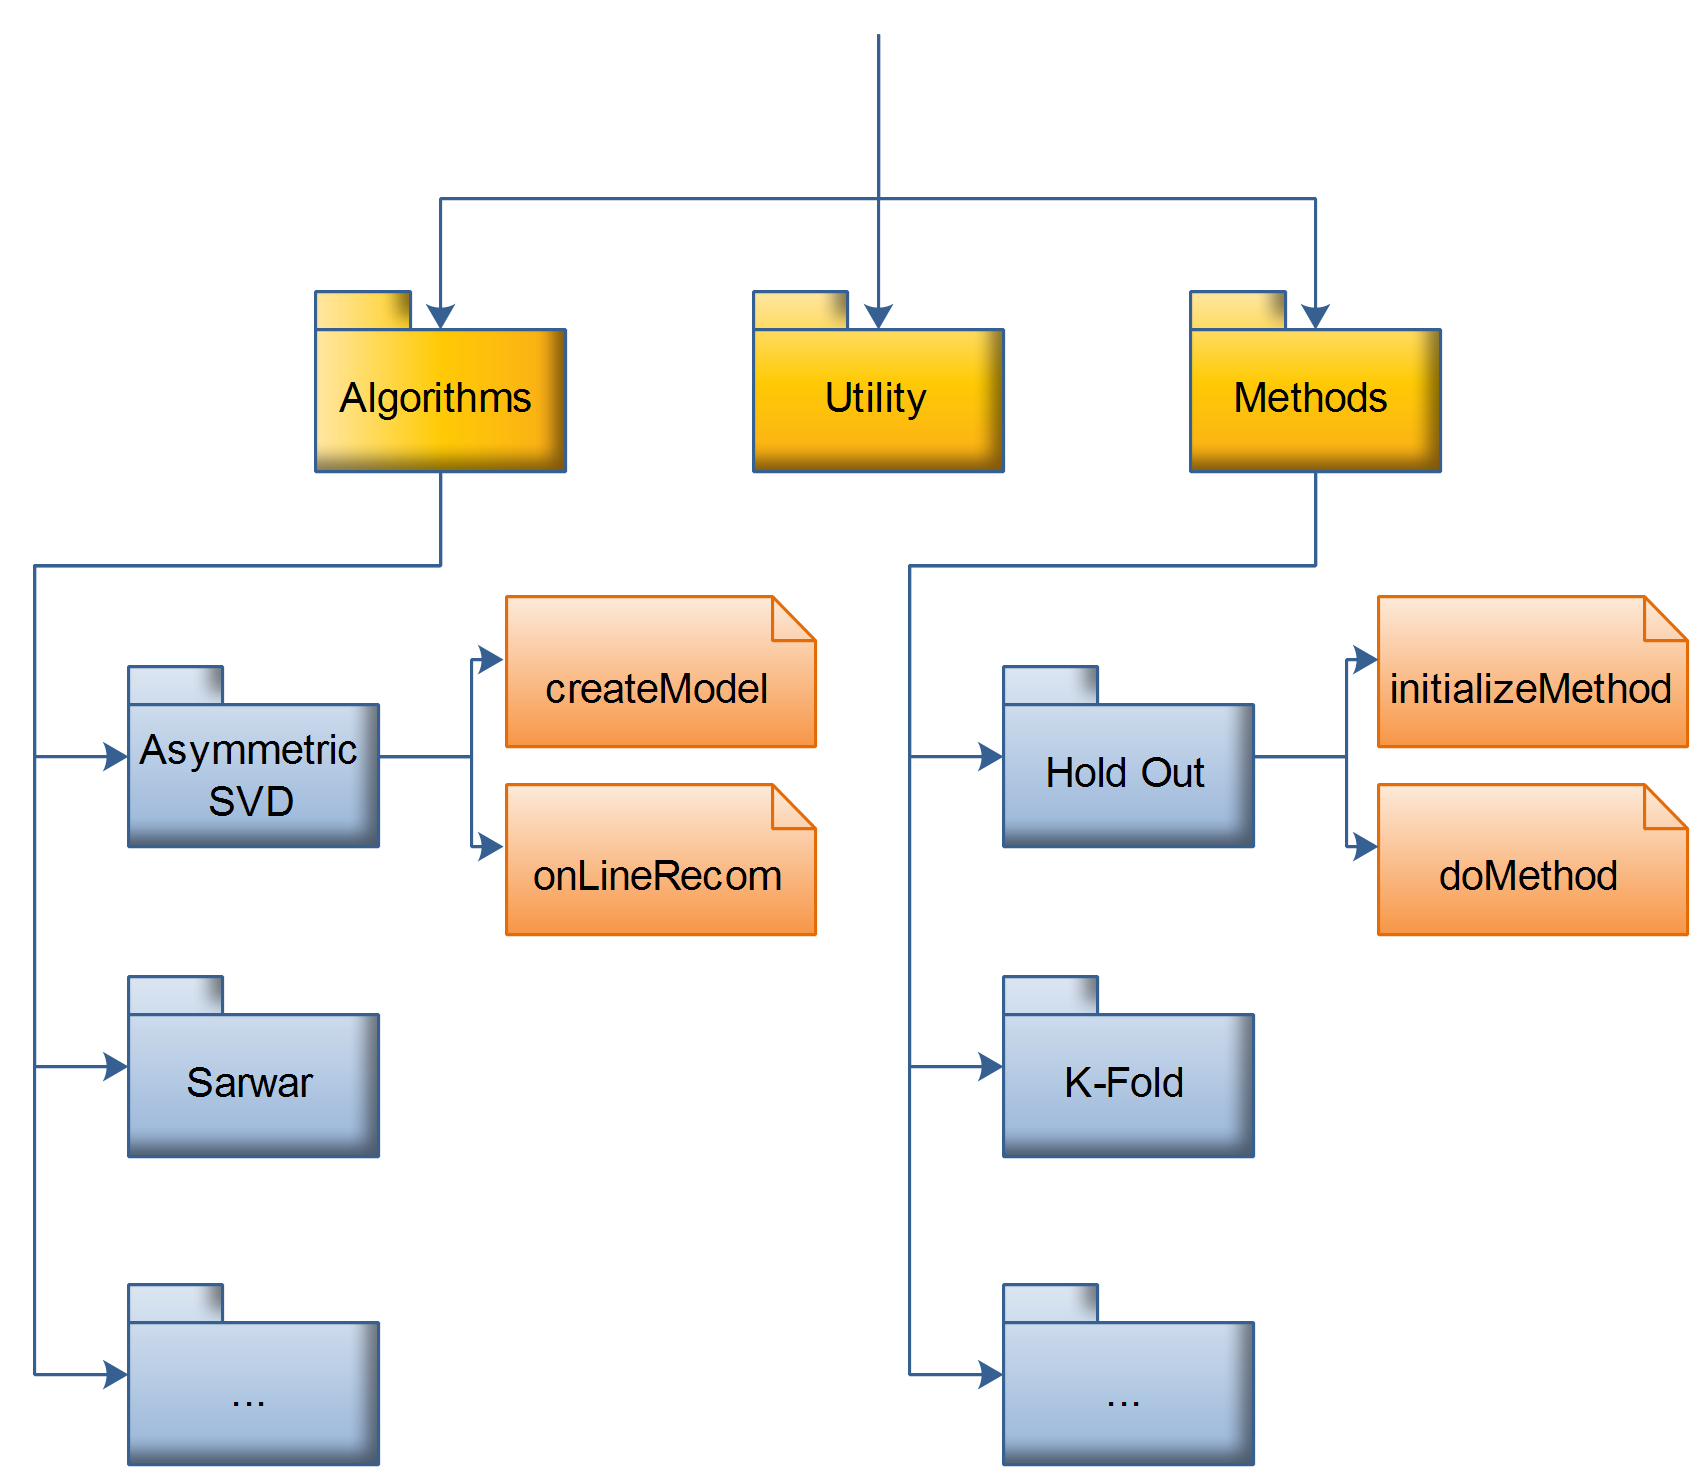
\includegraphics[scale=0.7]{./img/Cartelle}
	\end{center}
	\caption{Struttura del filesystem}
	\label{f:reing:dir}
\end{figure}

\begin{description}
	\item[Algorithms] raccoglie, uno per cartella, i vari algoritmi di raccomandazione. All'interno di queste cartelle sono presenti due file Matlab: 
	\begin{description}
		\item[createModel] si occupa della creazione del modello, prendendo come input la matrice \urm (di dimensione $ m \times n $) e una struttura di parametri aggiuntivi che servono per specificare alcune opzioni dei vari algoritmi. Tra questi parametri deve esserci \corsivo{Path}\nota{Questo parametro viene inserito in automatico dall'oggetto Recommendation.} che specifica il percorso della root della struttura dati e pu� anche esserci il parametro \corsivo{Model}: se � settato la funzione ritorna subito il contenuto di questo parametro, senza effettuare ulteriori controlli. Quest'opzione � stata aggiunta in quanto molto spesso la creazione del modello � computazionalmente talmente onerosa da rendere impossibili certi test, quindi questi vengono eseguiti utilizzando pi� volte il medesimo modello e abbreviando quindi i tempi di calcolo. L'output di questa funzione sar� il modello della raccomandazione, che verr� poi gestito dall'oggetto Recommendation stesso.
\begin{lstlisting}[style=Matlab, caption={Funzione createModel}, label=l:reing:strut:cm]
Model = createModel(URM, Parameters)
\end{lstlisting}
		\item[onLineRecom] si occupa di generare la lista di suggerimenti. Prende come input il modello creato in precedenza, il profilo utente (un vettore riga di lunghezza $ n $) e infine, come gi� visto per la createModel, una struttura di parametri aggiuntivi per modificare alcuni comportamenti dell'algoritmo. Come nel caso della createModel, anche qui deve esserci il parametro \corsivo{Path}. L'output di questa funzione � un vettore colonna di lunghezza $ m $ con i rating dei vari item.
\begin{lstlisting}[style=Matlab, caption={Funzione onLineRecom}, label=l:reing:strut:olr]
List = onLineRecom(UserProfile, Model, Parameters)
\end{lstlisting}
	\end{description}
	Ogni algoritmo ha le sue particolarit� e per questo il sistema non interviene mai sul modello della raccomandazione, ma si limita a passare il dato dalla funzione di creazione a quella di generazione della lista. Solamente i parametri di ingresso e la lista finale sono ""standardizzati'', tutto il resto � specifico da algoritmo ad algoritmo.
	\item[Methods] contiene le diverse metodologie di test che risultano divise in due funzioni:
	\begin{description}
		\item[initializeMethod] � la funzione che viene lanciata quando si vuol testare un algoritmo con un certo metodo. Contiene tutte le dovute inizializzazioni come preparare la matrice di Train e quella di Test. Al suo interno verr� richiamato il doMethod. Avr� come parametri di input la matice \urm, la matrice di Probe su cui fare il Train del test, l'algoritmo di raccomandazione che si vuole studiare e infine i vari parametri che si vogliono utilizzare, quelli del metodo in s�, quelli della createModel e infine quelli dell'onLineRecom. L'output sar� un oggetto con al suo interno i risultati del test secondo una determinata metrica (principalmente RMSE).
\begin{lstlisting}[style=Matlab, caption={Funzione initializeMethod}, label=l:reing:strut:im]
Result = initializeMethod(URM, URMProbe, Algorithm, MethodParameters, ModelParameters, OnLineParameters)
\end{lstlisting}
		\item[doMethod] contiene tutte le operazioni tipiche della metodologia di test. Per funzionare a dovere ha bisogno che gli siano passati tutta una serie di parametri che la inizializeMethod ha il compito di preparare. In alcuni metodi � possibile richiamare una funzione doMethod di un altro metodo di test. Gli input di questa funzione sono l'algoritmo da testare, la matrice \urm, la matrice di Train, il set dei test positivi e di quelli negativi e infine i parametri della createModel e dell'onLineRecom. L'output � un array con i test positivi e quelli negativi.
\begin{lstlisting}[style=Matlab, caption={Funzione doMethod}, label=l:reing:strut:dm]
[PositiveTests, NegativeTests] = doMethod(Algorithm, URM, URMTrain, PositiveTestSet, NegativeTestSet, ModelParameters, OnLineParameters)
\end{lstlisting}
	\end{description}
	Questa suddivisione � stata introdotta in quanto � possibile che un metodo utilizzi parte di un altro metodo per svolgere alcune funzioni.
	\item[Utility] contiene tutte quelle funzioni che servono a far funzionare i vari algoritmi e le funzioni di test. Al suo interno si possono trovare funzioni per la normalizzazione delle matrici, per il reshuffling e infine la libreria C che si occupa di velocizzare le operazioni pi� onerose. Si � scelto di inserire tutti i file in questa cartella per fare ordine, cosa che prima dell'intervento in oggetto a questo lavoro di tesi non era minimamente pensabile.
\end{description}

\section{Gli oggetti}
\label{c:reing:ogg}

Si passa ora all'esame dettagliato dei due oggetti principali del lavoro di reingegnerizzazione, \corsivo{Recommendation} e \corsivo{Test} che rappresentano anche i soli punti di contatto tra il sistema e l'utente: infatti tutte le interazioni avverranno attraverso questi wrapper mediante opportune API. Verranno anche presentati i metodi principali di questi oggetti, in modo da fornire un esempio di utilizzo.

\subsection{Recommendation}
\label{c:reing:ogg:rec}

Quest'oggetto � stato ideato partendo da una semplice idea: ogni istanza deve rappresentare un'esperienza di raccomandazione, quindi l'utente deve creare solamente un oggetto e continuare ad usarlo memorizzando al suo interno dati finch� non ha finito la raccomandazione completa. In questo modo l'utente non si trova ad avere memorizzate troppe istanze dell'oggetto stesso, col risultato di risparmiare memoria e soprattutto rendere ordinato il workspace.

L'utente deve inoltre poter scegliere tranquillamente quale algoritmo utilizzare, e quindi non doversene pi� interessare: � l'oggetto che andr� a costruire il modello e creer� la lista di raccomandazioni secondo quel determinato algoritmo. \`E anche possibile modificare l'algoritmo scelto, ma poi sar� necessario ricreare il modello in quanto potrebbero nascere delle incompatibilit�, basti pensare a due algoritmi che utilizzano modelli differenti.

Altra particolarit� di quest'oggetto � non salvare la matrice \urm: essa viene tenuta in memoria nell'ambiente base di Matlab, in modo da non pesare all'interno dell'oggetto. In questo modo l'accesso risulta essere pi� rapido. Si � voluto cercare di portare su Matlab il concetto dei puntatori del linguaggio C, ma non esistendo un costrutto del genere si � iniziato a lavorare differenziando i workspace. A tal scopo all'interno dell'oggetto viene salvato solamente il nome della matrice, che risiede fisicamente nell'ambiente di base.

Infine si � cercato di memorizzare tutti i risultati delle raccomandazioni eseguite: in questo modo si pu� accedere rapidamente nel caso di Reshuffling e di test in cui si vogliono avere a disposizione le ultime liste create. Inoltre quest'operazione non � computazionalmente troppo onerosa in quanto si tratta semplicemente di vettori colonna, seppur di grandi dimensioni.

Si prosegue quindi con l'analisi dei diversi metodi e attributi di quest'oggetto.

\subsubsection{Attributi Privati}
\label{c:reing:ogg:rec:pri}

Sono stati protetti in scrittura poich� non risulta essere d'interesse modificarne il valore. Sar� invece importante potervi accedere in lettura (soprattutto a uno dei tre).

\begin{description}
	\item[Model] � il modello utilizzato. Viene creato da un apposito metodo. Teoricamente potrebbe essere protetto anche in lettura in quanto non � di enorme interesse conoscerne la forma, ma visto che per alcune fasi di debug pu� risultare interessante leggerne il contenuto, si preferisce lasciarlo pubblico in lettura.
	\item[Path] � una stringa contenente il percorso assoluto della root della nostra struttura di cartelle. Serve alle varie funzioni per includere le diverse cartelle da cui prendere file utili (come la cartella delle Utility). Viene impostato dal costruttore dell'oggetto e in seguito non viene pi� modificato. Viene aggiunto a tutti i parametri e quindi passato in tutte le funzioni di creazione del modello e creazione della lista.
	\item[Result] � un array contenente un oggetto per ogni raccomandazione. Questo oggetto � organizzato nel seguente modo:
	\begin{description}
		\item[Result.List] � la lista vera e propria, cos� come esce dalla funzione di raccomandazione. Contiene tutti i voti dati ai vari elementi.
		\item[Result.Ranking] � un array contenente le chiavi degli elementi di Result.List ordinati in modo decrescente, quindi il primo valore � la chiave dell'elemento col voto maggiore.
		\item[Result.UserProfile] � il profilo utente utilizzato per generare la raccomandazione. Nel caso in cui il risultato provenga dalla funzione di antireshuffling e non da una raccomandazione vera e propria, � un array contenente i due profili utenti associati alle liste su cui � stato applicato l'antireshuffling.
	\end{description}
\end{description}

\subsubsection{Attributi Pubblici}
\label{c:reing:ogg:rec:pub}

I seguenti attributi, possono essere soggetti a modifiche da parte dell'utente. Proprio per questo sono pubblici, bench� la loro modifica sia soggetta a vincoli, anche molto stringenti per quanto riguarda uno di essi.

\begin{description}
	\item[Algorithm] � l'algoritmo che si utilizza per generare la raccomandazione. \`E una stringa e deve corrispondere alla cartella in cui sono contenuti i file con le funzioni utilizzate. Non � necessario memorizzare tutti i nomi, poich� in caso d'errore il sistema � in grado di stampare schermo il nome di tutti gli algoritmi disponibili. Questa propriet� pu� essere modificata solamente prima di creare il modello della funzione: in caso contrario verr� stampato un messaggio d'errore e l'algoritmo rimarr� il medesimo.
	\item[URM] � una stringa che corrisponde al nome della variabile, nell'ambiente \corsivo{base}, che costituisce la matrice \urm. Come per l'algoritmo, anche questa stringa non pu� essere modificata dopo la creazione del modello. Si occupa in automatico di caricare le variabili indicate quando la stringa passata corrisponde a un file nel workspace.
\end{description}

\subsubsection{Metodi}
\label{c:reing:ogg:rec:met}

In questa fase di esamineranno i metodi che permettono all'utente di interagire con l'oggetto per creare il modello, la raccomandazione e per altre funzionalit�. Tutti i metodi che verranno presentati sono pubblici in quanto non c'� alcuna necessit� di creare metodi privati poich�, come ripetuto pi� volte in questa trattazione, l'oggetto non � nient'altro che un wrapper. Per completezza � opportuno informare il lettore che in seguito i parametri opzionali per i metodi saranno posti tra tramite parentesi quadre.

\begin{description}
	\item[Recommendation] � il costruttore dell'oggetto. Prende come parametri il nome della matrice \urm da utilizzare e il nome dell'algoritmo. L'assegnazione del nome della variabile contenente la matrice e dell'algoritmo sono soggetti a limitazioni nel caso in cui non esista o la variabile o il file contenente la matrice \urm, oppure non esista la cartella indicata come algoritmo da utilizzare. Nel caso queste assegnazioni non vadano a buon fine, l'oggetto viene comunque creato, ma con i campi summenzionati vuoti. Sar� poi compito dell'utente andare a riempirli prima di creare il modello.
\begin{lstlisting}[style=Matlab, caption={Funzione costruttrice dell'oggetto Recommendation}, label=l:reing:met:rec]
R = Recommendation(URM, Algorithm)
\end{lstlisting}
	\item[createModel] serve per creare il modello della funzione. Come � facilmente intuibile, controlla innanzitutto che siano settati l'algoritmo da utilizzare e la matrice URM. Come input prende una struttura di parametri che poi saranno passati alla funzione di creazione vera e propria. Dal momento che molte funzioni di creazione del modello necessitano di altre funzioni ""ausiliarie'', alla struttura di parametri viene aggiunto \corsivo{Path}. E, una volta creato, il modello viene memorizzato nell'attributo privato dell'oggetto.
\begin{lstlisting}[style=Matlab, caption={Metodo per la costruzione del modello}, label=l:reing:met:cm]
createModel([Parameters])
\end{lstlisting}
	\item[onLineRecom] si occupa della creazione e della memorizzazione della lista di raccomandazioni. Ha due parametri in ingresso: il vettore col profilo utente e la solita struttura di parametri da usare nella funzione di generazione dei suggerimenti. Come visto per la createModel, anche qui viene aggiunto il parametro indicante il percorso sul filesystem. L'output del metodo � la lista contenente le votazioni di ogni singolo elemento. Nell'oggetto viene inserita una voce all'attributo \corsivo{Result}, contenente tutte le informazioni viste al punto \ref{c:reing:ogg:rec:pri}.
\begin{lstlisting}[style=Matlab, caption={Metodo per la creazione della lista di raccomandazioni}, label=l:reing:met:olr]
List = onLineRecom(UserProfile[, Parameters])
\end{lstlisting}
	\item[antiReshuffling] si prende in carico l'esecuzione dell'antireshuffling su due risultati ottenuti con la onLineRecom. I parametri di ingresso sono tre: il primo indice dell'array Result contenuto nell'oggetto (alternativamente pu� essere specificato un profilo utente su cui eseguire la raccomandazione), il secondo indice (anche qui si pu� specificare un profilo utente) e infine una struttura di parametri. Si pu� scegliere di non specificare tutti gli input operando quindi nei seguenti modi:
	\begin{itemize}
		\item se non vengono passati i parametri si esegue la funzione tra gli ultimi due risultati;
		\item se si specifica un solo indice (o vettore utente) viene eseguito l'antireshuffling tra questo e l'ultimo;
		\item se si specifica solo una struttura di parametri si considerano gli ultimi due risultati e si passano i parametri specificati;
		\item se vengono passati due indici (o vettori utente) si esegue l'antireshuffling tra quei due valori;
		\item se vengono passati un indice e una struttura di parametri si produce come risultato la combinazione del risultato indicato e dell'ultimo, passando alla funzione i parametri.
	\end{itemize}
	L'output del metodo � la nuova lista di raccomandazioni, inoltre viene memorizzata nell'attributo Result la lista pi� altre informazioni, come visto nel gi� citato punto \ref{c:reing:ogg:rec:pri}.
\begin{lstlisting}[style=Matlab, caption={Metodo per la funzione di antireshuffling}, label=l:reing:met:ar]
List = antiReshuffling([Index1[, Index2[, Parameters]]])
\end{lstlisting}
	\item[export] si occupa, dell'esportazione dei risultati su un file di testo. Viene utilizzata la convenzione \csv\nota{Coma Separated Values, ovvero valori separati da una virgola o pi� in generale da un limitatore.} utilizzando un \# per separare i diversi valori e una | per i campi. La funzione prende come input il file su cui memorizzare e gli indici (che possono essere passati sia come valori, sia come array) dei risultati da esportare. Se non viene specificato l'indice del risultato da esportare, la funzione agir� sull'ultimo creato.
\begin{lstlisting}[style=Matlab, caption={Metodo per l'esportazione dei risultati}, label=l:reing:met:ex]
export(File[, Index])
\end{lstlisting}
\end{description}

\subsection{Test}
\label{c:reing:ogg:test}

Quest'oggetto si occupa di testare un algoritmo secondo diverse metodologie. Il test di per s� viene pensato come qualcosa di automatico, in cui l'utente pu� cambiare i parametri in modo da effettuare una procedura adatta alle proprie esigenze.

Come gi� visto per le raccomandazioni, anche il test � un oggetto di cui basta anche solo un'istanza per poter operare: i risultati vengono salvati, secondo diverse metriche, all'interno dell'oggetto stesso, cos� che si possano eseguire diverse prove con algoritmi differenti o addirittura con metodologie differenti. 

Ovviamente il suo funzionamento � legato a quello dell'oggetto Recommendation poich� tutte le raccomandazioni sono affidate a quest'ultimo. Attraverso un passaggio di parametri adeguato, l'utente pu� intervenire in qualsiasi punto della raccomandazione, in modo da avere il pieno controllo e gestire, ad esempio, spazi latenti differenti per pi� prove con lo stesso metodo.

\subsubsection{Attributi Privati}
\label{c:reing:ogg:test:pri}

Analogamente all'oggetto Recommendation, anche qui gli attributi privati sono riservati a informazioni che l'utente non deve modificare, ma che ugualmente possono essere letti.

\begin{description}
	\item[Path] � il percorso assoluto dell'M-file contenente l'oggetto in questione. Serve, come visto in precedenza, per includere le funzioni ausiliarie e i metodi di testing. Viene settato in automatico in fase di inizializzazione dell'oggetto.
	\item[Result] � il contenitore dove vengono memorizzati tutti i risultati dei vari test fatti tramite l'oggetto istanziato. \`E un array di struct dove ogni voce rappresenta una metrica (quella pi� usata � l'RMSE, ma ne esistono altre).
\end{description}

\subsubsection{Attributi Pubblici}
\label{c:reing:ogg:test:pub}

Queste propriet� dell'oggetto, diversamente dalle precedenti, possono essere modificate. Gli attributi, questi devono sottostare a vincoli per la buona riuscita dell'algoritmo di test, come verr� pi� esplicitamente esaminato nelle singole spiegazioni.

\begin{description}
	\item[Algorithm] � l'algoritmo utilizzato per generare le raccomandazioni e i modelli. Deve essere uguale al nome della cartella in cui sono memorizzate le sue funzioni. Nel caso in cui non ci si ricordi del nome esatto, il sistema stamper� a video l'elenco degli algoritmi disponibili.
	\item[Method] rappresenta la metodologia di test scelta. Similmente all'algoritmo, anche questa stringa deve coincidere con una determinata cartella. Anche per questo attributo non � necessario ricordare tutti i nomi perch� l'oggetto stamper� a video tutte le metodologie disponibili.
	\item[URM] � il nome della variabile da usare per la matrice URM. Se il nome specificato � quello di un file \corsivo{.mat} o \corsivo{.mm}, il sistema andr� in automatico a leggerlo dal filesystem e lo importer� nel workspace.
	\item[URMProbe] � la matrice usata per il testing vero e proprio. Viene memorizzata solamente la stringa corrispondente e quindi caricata ogni volta dalla memoria.
\end{description}

\subsubsection{Metodi}
\label{c:reing:ogg:test:met}

A differenza dell'oggetto Recommendation, Test non ha molti metodi al suo interno: � facilmente intuibile che per generare una raccomandazione necessitano diversi passi, mentre � sufficiente far girare un test per avere dei risultati. Avremo quindi solamente i metodi indispensabili. Questa scelta � anche suggerita dal fatto che s'� voluto semplificare al massimo l'oggetto, lasciando tutta la complessit� alle funzioni che gestiscono le metodologie di testing e soprattutto alla scelta dei parametri. Sar� poi l'utente a utilizzare pi� volte lo stesso oggetto per avere test particolari.

\begin{description}
	\item[Test] � il costruttore dell'oggetto. Prende come parametri di input le due matrici da utilizzare, \urm e Probe, l'algoritmo per la raccomandazione e il metodo di test. Nel caso in cui una di queste assegnazioni non sia corretta (ad esempio si sceglie un algoritmo inesistente) l'oggetto viene creato ugualmente, ma manca dell'attributo settato. Successivamente quando si cercher� di utilizzare un altro metodo verr� restituito un messaggio d'errore.
\begin{lstlisting}[style=Matlab, caption={Funzione costruttrice dell'oggetto Test}, label=l:reing:met:tst]
T = Test(URM, URMProbe, Algorithm, Method)
\end{lstlisting}
	\item[fire] si occupa di far partire il metodo di test, quindi di lanciare la funzione initializeMethod contenuta nella cartella \corsivo{Method} scelta. Prende in ingresso i tre diversi tipi di parametri: quelli del metodo di test, quelli della funzione che crea il modello e quelli della funzione che genera la raccomandazione vera e propria. Questi tre input sono tutti facoltativi in quanto si pu� optare per l'utilizzo dei parametri di default. L'output della funzione sar� il risultato ottenuto, che verr� anche salvato come ultima voce dell'array Result, attributo dell'oggetto istanziato.
\begin{lstlisting}[style=Matlab, caption={Metodo per lanciare il test}, label=l:reing:met:fr]
Result = fire([MethodParameters[, ModelParameters[, OnLineParameters]]])
\end{lstlisting}
\end{description}

\section{Use Cases}
\label{c:reing:uc}

La semplicit� d'uso � stato il filo conduttore di tutta l'implementazione della piattaforma in esame. Proprio per questo motivo vengono ora presentati i casi d'uso che rispecchiano una fruizione tipica dell'applicazione.

\begin{figure}
	\begin{center}
		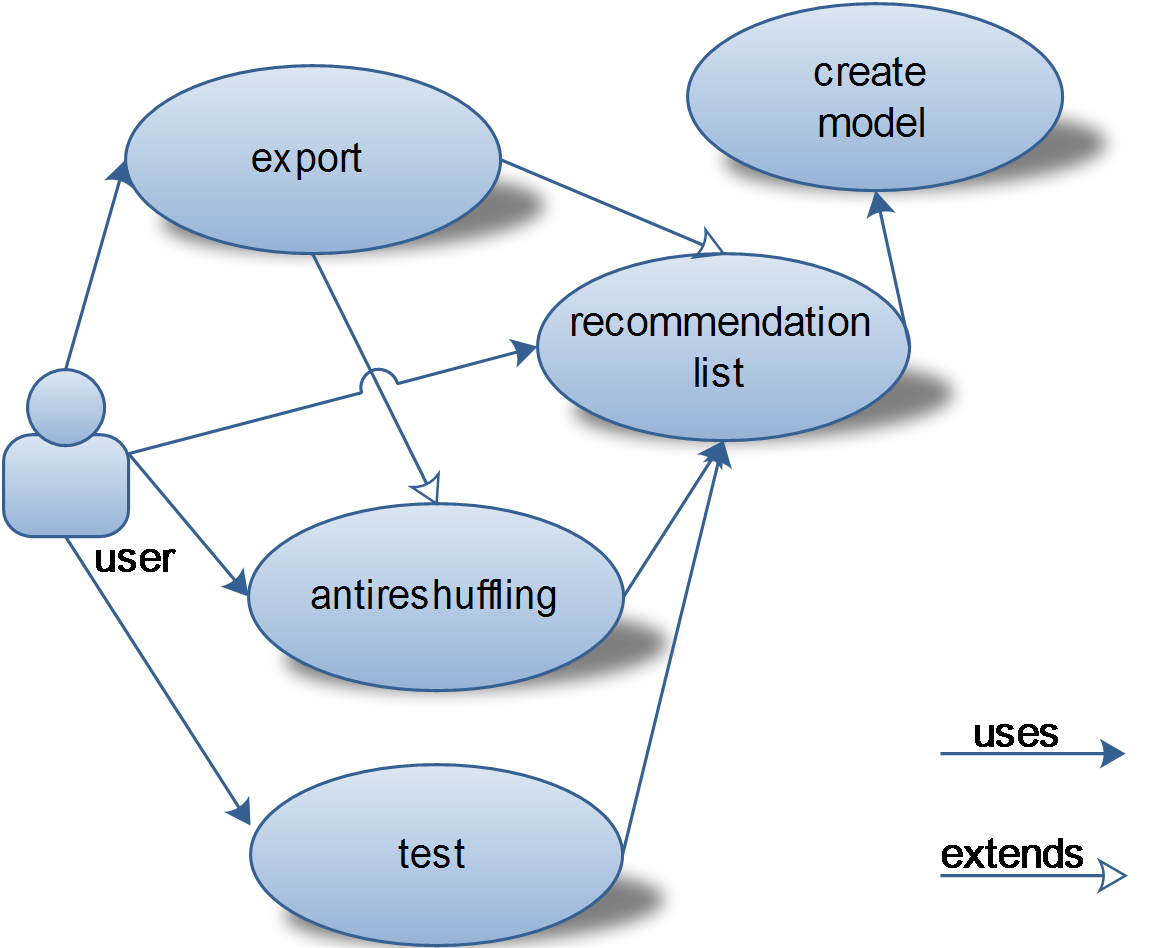
\includegraphics[scale=1]{./img/UseCases}
	\end{center}
	\caption{Gli use cases dell'applicazione}
	\label{f:reing:uc}
\end{figure}

\subsection{Generazione della lista di raccomandazione}
\label{c:reing:uc:rec}

\begin{figure}
	\begin{center}
		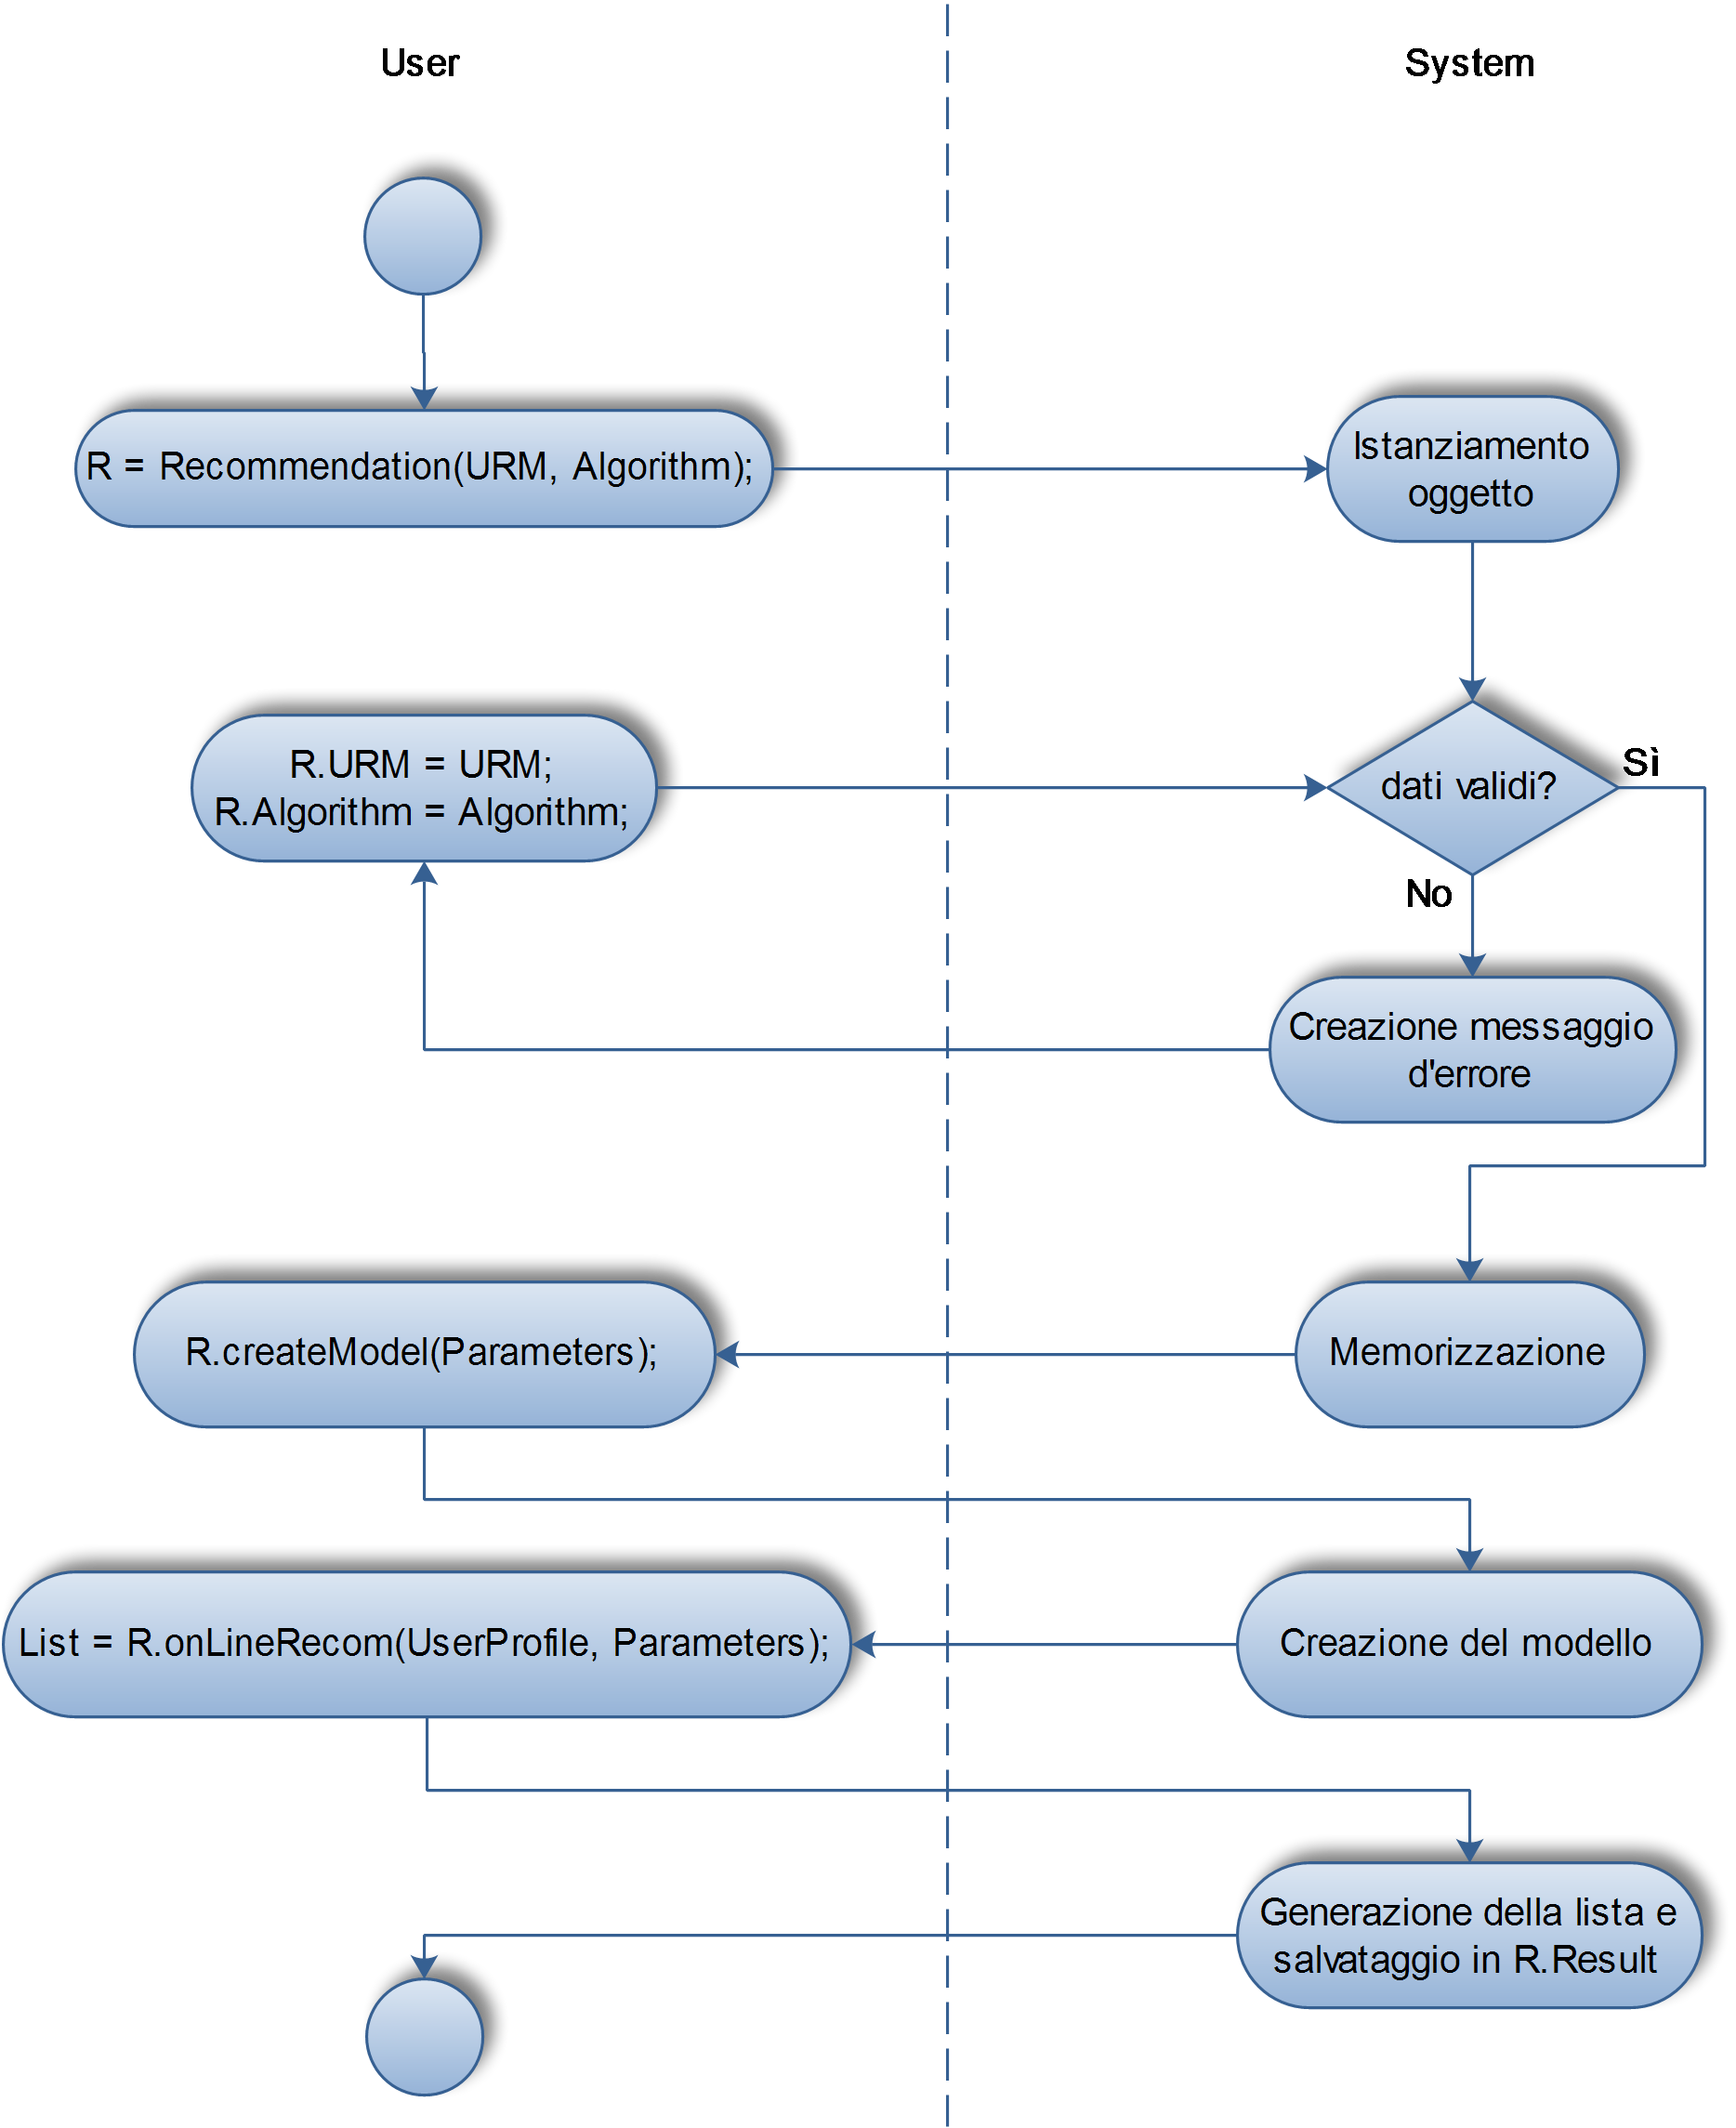
\includegraphics[scale=0.9]{./img/UseCase_RecList}
	\end{center}
	\caption{Use Case: generazione della lista di raccomandazione}
	\label{f:reing:uc:rec}
\end{figure}

Per generare un suggerimento bisogna interagire con l'oggetto Recommendation. I passaggi da svolgere sono pochi:

\begin{itemize}
	\item si istanzia l'oggetto passando come parametri del costruttore la matrice \urm e l'algoritmo scelto. Il sistema alloca lo spazio in memoria per l'oggetto e quindi controlla che i due input siano corretti; devono essere validi sia il nome della variabile che rappresenta la matrice, sia l'algoritmo di raccomandazione. Qualora non si verifichino queste condizioni, viene restituito un messaggio d'errore: l'oggetto � gi� stato istanziato e quindi bisogna procedere a settare gli attributi direttamente, senza ripassare dal costruttore. Quando i valori inseriti risultano essere idonei il sistema procede alla memorizzazione degli stessi.
	\item l'utente richiama il metodo che crea il modello. Il sistema va a cercare sul filesystem la funzione corrispondente e quindi la esegue, andando poi a memorizzare il risultato nell'attributo Model dell'oggetto.
	\item attraverso un profilo utente viene richiesta la generazione della lista di raccomandazione che successivamente � salvata nell'array Result in modo da poter essere riutilizzata in seguito.
\end{itemize}

\subsection{Esportazione della raccomandazione}
\label{c:reing:uc:exp}

\begin{figure}
	\begin{center}
		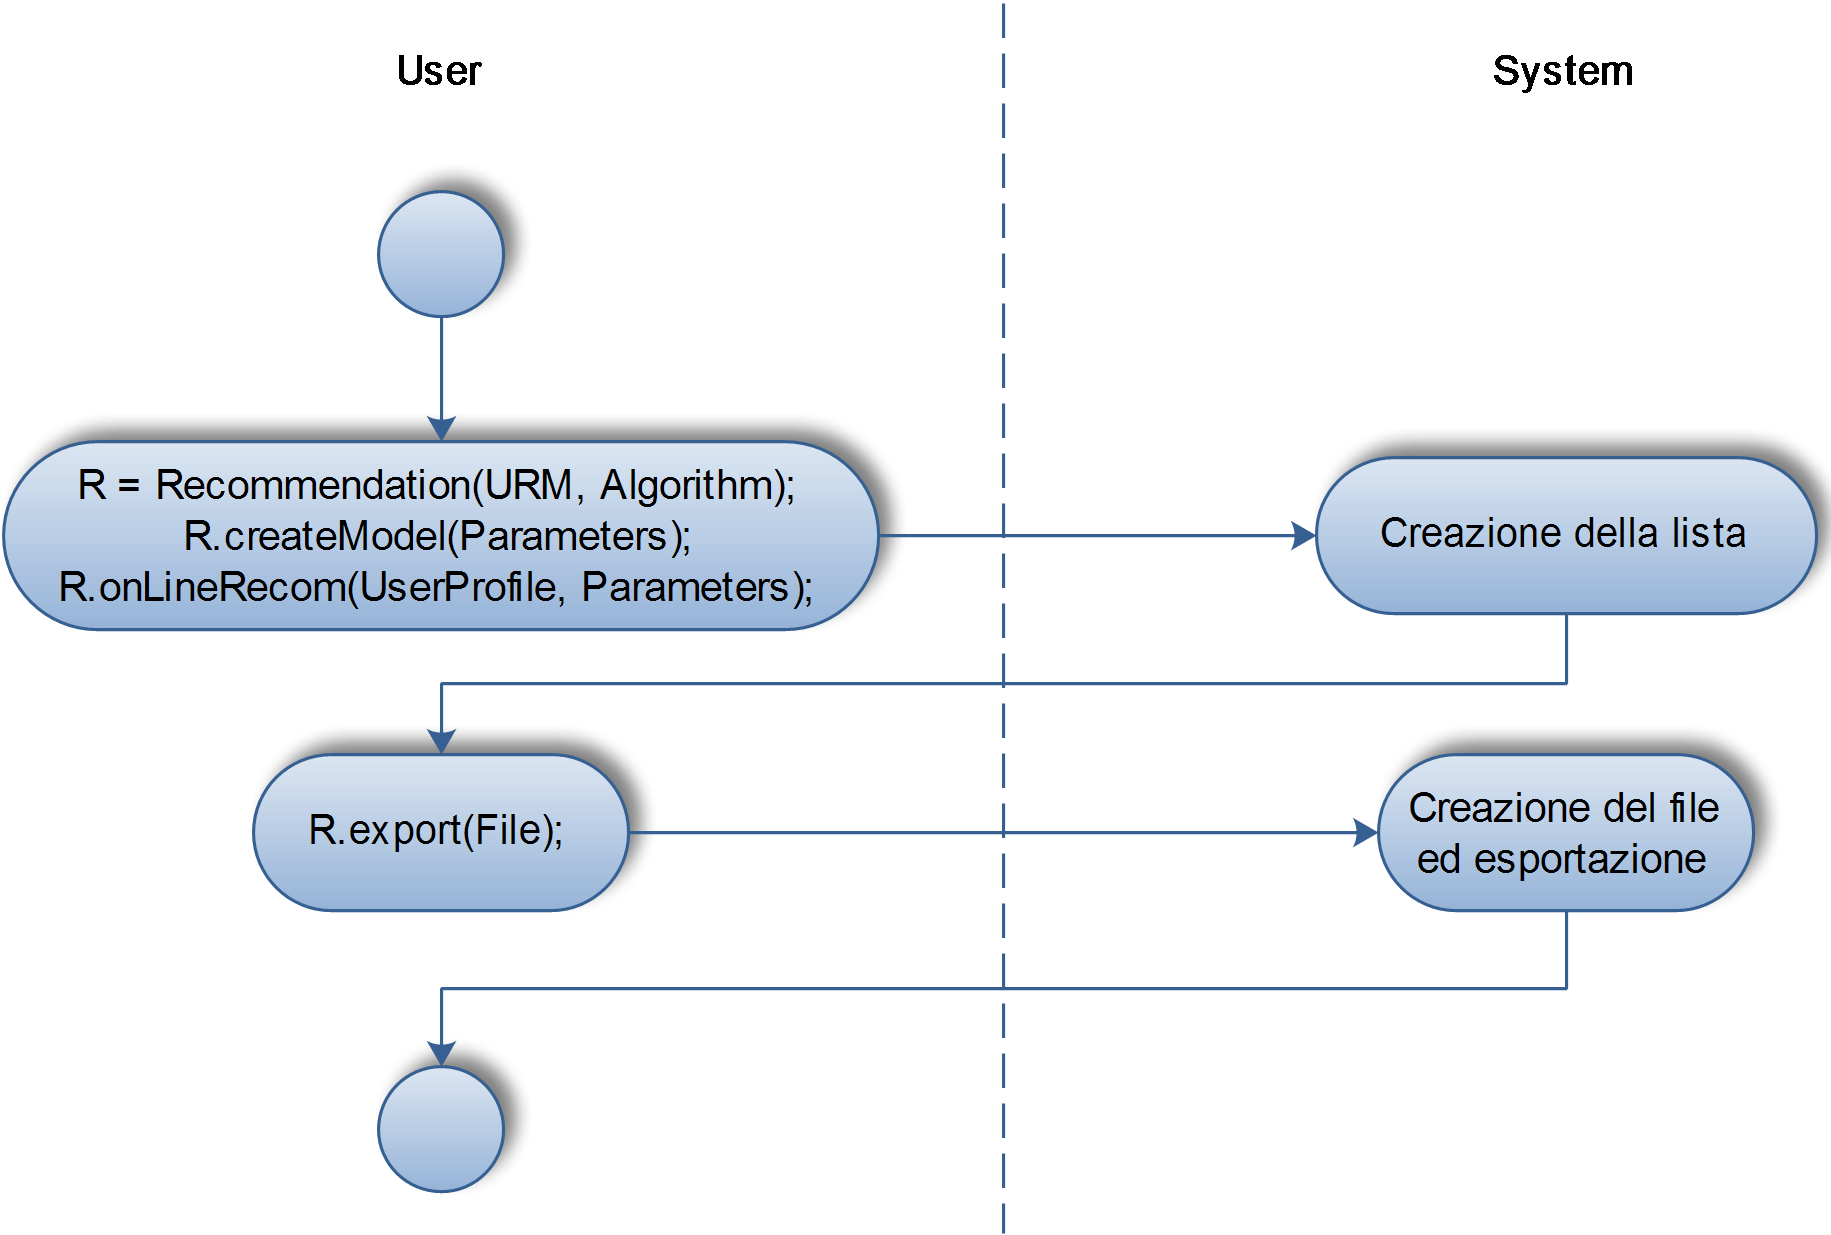
\includegraphics[scale=0.9]{./img/UseCase_Export}
	\end{center}
	\caption{Use Case: esportazione della raccomandazione}
	\label{f:reing:uc:exp}
\end{figure}

Ogni lista di suggerimenti pu� essere esportata in formato testale. Per far ci� � sufficiente:

\begin{itemize}
	\item creare la raccomandazione con i passaggi visti in precedenza.
	\item richiamare il metodo di export indicando su quale file debba essere memorizzata la stringa rappresentante la lista. Si pu� anche specificare quale dei tanti risultati esportare mediante l'uso di un array di indici.
\end{itemize}

\subsection{Antireshuffling}
\label{c:reing:uc:anti}

\begin{figure}
	\begin{center}
		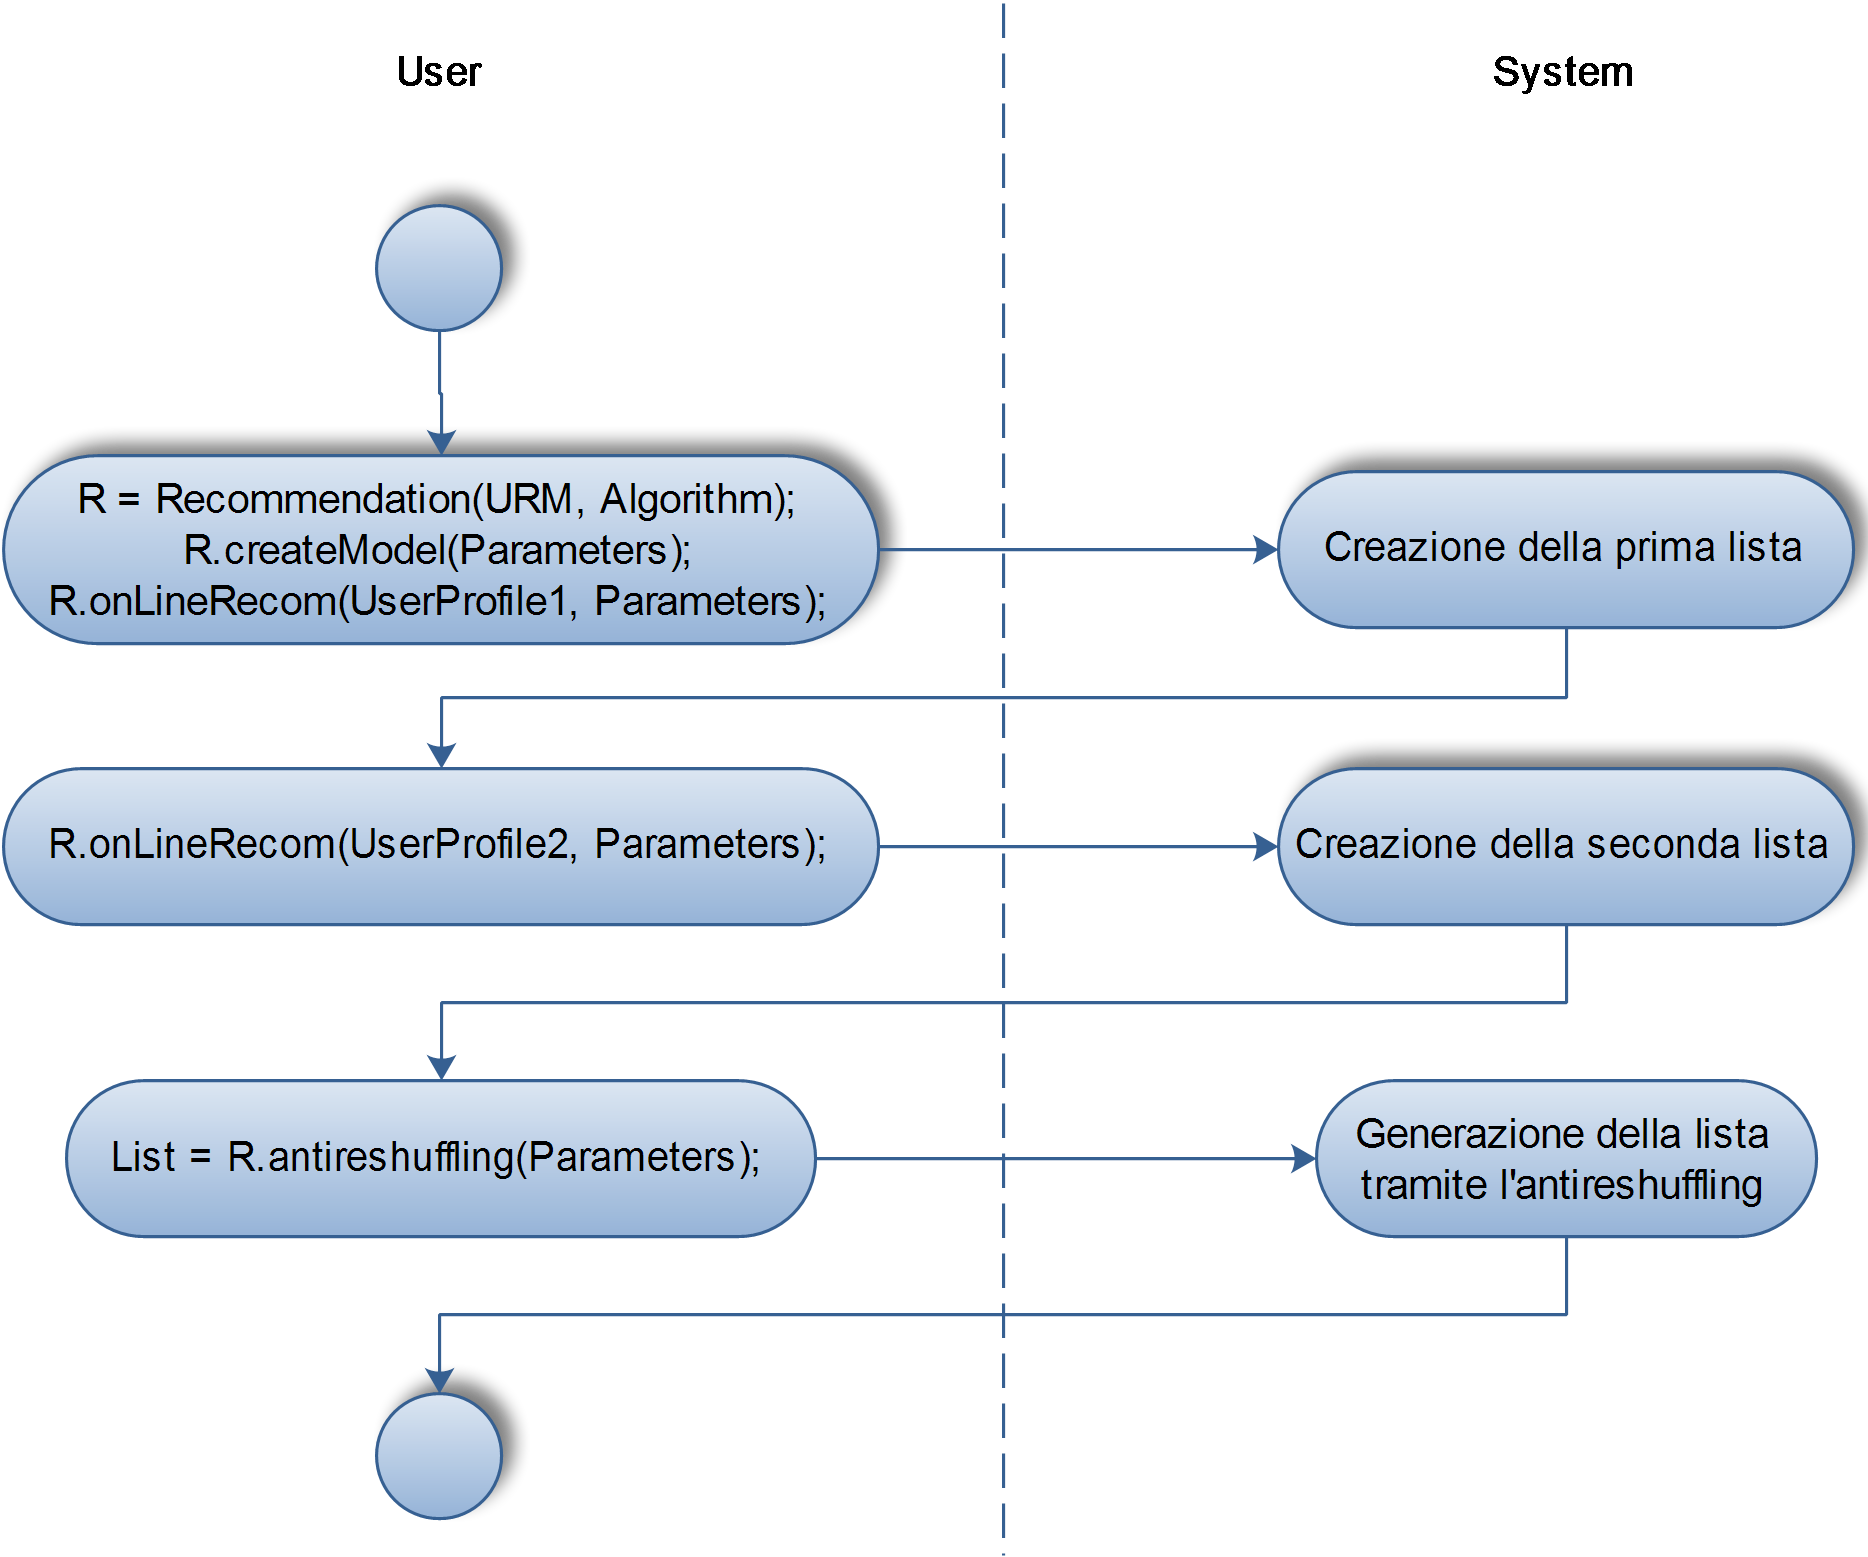
\includegraphics[scale=0.9]{./img/UseCase_Antireshuffling}
	\end{center}
	\caption{Use Case: antireshuffling}
	\label{f:reing:uc:anti}
\end{figure}

Si esamina ora la creazione di una lista di raccomandazioni tramite la tecnica di antireshuffling. Per far ci� bisogna prima generare due diverse liste di suggerimenti:

\begin{itemize}
	\item si costruisce la prima lista inserendo un profilo utente di un momento prefissato. La lista conseguente viene memorizzata nell'array Result.
	\item si inserisce un secondo profilo utente che genera una nuova lista di raccomandazioni. Anche questa viene automaticamente salvata nell'attributo Result dell'oggetto.
	\item si richiama quindi la funzione di antireshuffling che, prese le ultime due liste generate, calcola la risultante. Questa viene sia restituita come output della funzione, sia memorizzata nell'array Result per essere eventualmente utilizzata in seguito.
\end{itemize}

\subsection{Esecuzione di un test}
\label{c:reing:uc:test}

\begin{figure}
	\begin{center}
		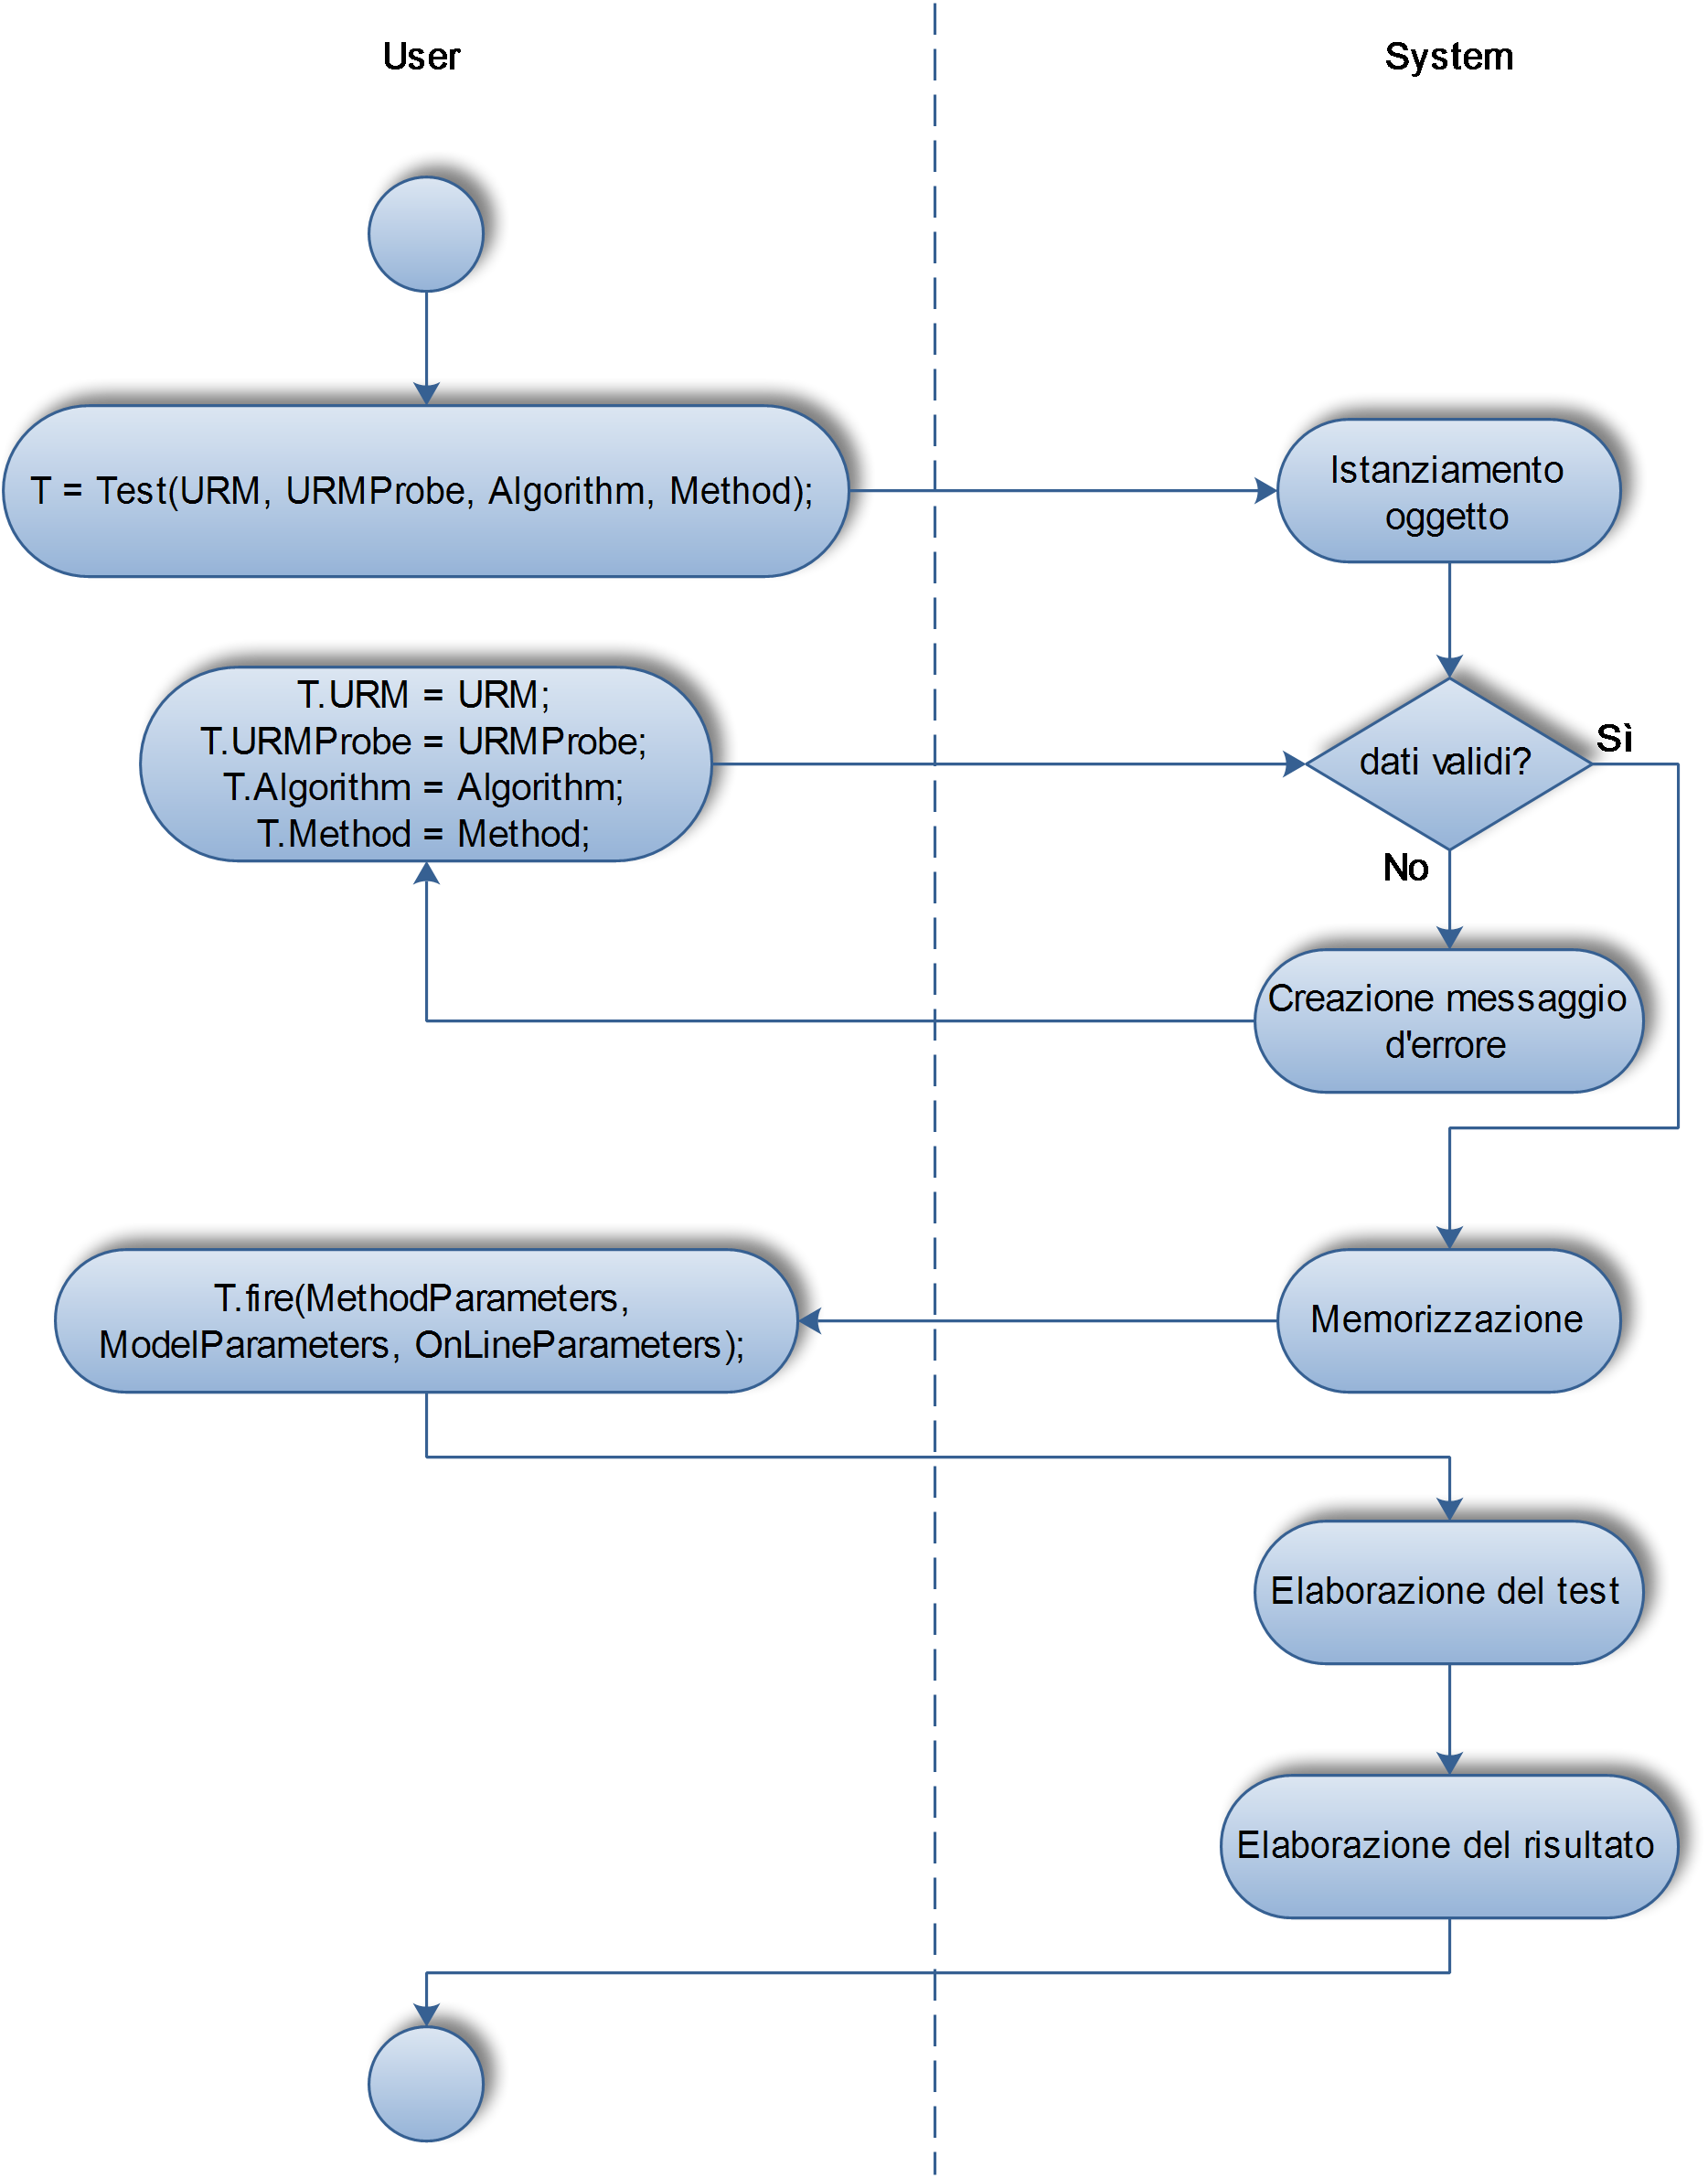
\includegraphics[scale=0.9]{./img/UseCase_Test}
	\end{center}
	\caption{Use Case: esecuzione di un test}
	\label{f:reing:uc:test}
\end{figure}

In questo caso pratico si usa l'oggetto Test. Anche in questo caso l'interazione col sistema � molto semplice e intuitiva:

\begin{itemize}
	\item prima di tutto si inizializza l'oggetto Test passando come parametri le due matrici \urm e Probe, il nome dell'algoritmo di raccomandazione che si vuole utilizzare e la metodologia scelta. Il sistema quindi allocher� lo spazio in memoria e verificher� la correttezza dei dati: le matrici devono esistere nell'ambiente di base (o alternativamente come file nel filesystem), l'algoritmo e la metodologia devono essere validi. Nel caso in cui almeno uno di questi parametri non sia corretto viene restituito un messaggio d'errore e l'utente deve provvedere alla correzione manuale dell'attributo. Quando non ci sono pi� problemi, ogni attributo viene memorizzato.
	\item si richiama il metodo che fa partire il test, passando come input i vari parametri da utilizzare per la metodologia di test, per la creazione del modello e per la generazione della lista di suggerimenti. Il sistema processer� tutto quanto e, dopo aver svolto l'intero test, creer� un oggetto contenente i risultati memorizzandolo nell'array Result.
\end{itemize}
\chapter{Integrazione in un Sistema Reale}
\label{c:int}

Tutto quanto visto finora non � mai stato messo a confronto con un sistema reale: potrebbe praticamente servire una piattaforma simile fuori dall'ambito accademico? Quali sono le sue limitazioni e quali i suoi punti di forza? 

Si cercher� ora di sottoporre questo sistema alle diverse esigenze che si possono incontrare al di fuori di un contesto di testing.

\section{Integrazione}
\label{c:int:int}

Il principio cardine di tutta la piattaforma � la facilit� di implementazione: la struttura a oggetti permette una gestione semplice di tutto il flusso di dati in quanto non vengono allocate troppe variabili per memorizzare i vari stati dell'applicazione. 

Anche i metodi sono stati pensati per rendere intuitivo l'utilizzo: non ne esistono di superflui, ognuno ha una sua precisa funzione. Tramite essi si pu� accedere a tutte le funzionalit� dell'oggetto, senza dover avere una conoscenza approfondita degli attributi e dei parametri.

L'utente avanzato, invece, sar� interessato a tutti i diversi parametri per agire direttamente sul metodo: per esempio, la creazione di un modello pu� avvenire in modo differente in base alle opzioni che vengono passate. Questa gestione personalizzata pu� influire positivamente sulla riuscita di una particolare raccomandazione e proprio per questo durante l'implementazione si � cercato di tenere sempre in considerazione tutti i possibili parametri in modo da lasciare all'utente l'opzione di variare alcune condizioni. Esemplificativo � il passaggio del modello ai metodi che lo creano: in questo modo la funzione ritorna subito evitando calcoli inutili.

\section{Ampliamento e API}
\label{c:int:api}

In campo informatico l'evoluzione � rapidissima ed � estremamente difficoltoso stare al passo con questo susseguirsi di aggiornamenti e nuove idee. Proprio per questo motivo la piattaforma � stata creata a moduli: ogni algoritmo di raccomandazione e ogni metodologia � una funzione a se stante, richiamata dal metodo, sulla quale non ci sono particolari controlli, a parte richiedere un output e certi parametri di input. Questa soluzione � stata adottata per consentire una libert� totale all'ampliamento del sistema: implementare un nuovo algoritmo � facilissimo e l'operazione viene riconosciuta subito dall'oggetto.

Analogamente s'� scelto di non creare costrutti rigidi per i parametri dei singoli metodi: si possono passare anche oggetti incredibilmente complessi, sta poi alla funzione chiamata saperli gestire. Esemplare da questo punto di vista � il modello della raccomandazione: all'oggetto non interessa come venga creato o come sia strutturato. \`E solo memorizzato e quindi passato alla funzione che genera la lista di suggerimenti. Quest'assenza di controllo rende possibile la gestione della struttura dati da parte dell'implementatore, che per questo motivo non � pi� costretto a ""nascondere'' i propri oggetti dentro strutture articolate come si era soliti fare in alcuni punti della vecchia applicazione.

\section{Risorse Computazionali}
\label{c:int:ris}

La costruzione del modello � una fase computazionalmente molto impegnativa: il calcolatore deve analizzare e operare su migliaia di dati e il motore di Matlab non ne � sempre all'altezza. Le maggiori difficolt� si sono riscontrate con le matrici, in quanto la maggior parte degli algoritmi le analizza una riga alla volta: il programma, al contrario, le memorizza per colonne, e quindi risulta molto dispendioso estrarre un singolo elemento da una colonna. Proprio per questo una prima ottimizzazione si � verificata introducendo le matrici trasposte, ma ancora in alcune fasi il sistema risulta essere troppo lento.

Le operazioni pi� lunghe sono state implementate in \corsivo{C} in quanto Matlab supporta l'esecuzione di funzioni in questo linguaggio in modo quasi nativo (� sufficiente disporre di un compilatore sulla propria macchina). In questo modo il tempo di esecuzione di alcuni metodi � ridotto drasticamente, rendendo possibile anche la fase di testing (che richiede svariate creazioni di un modello) in tempi ragionevoli.

Nonostante questo, per�, risulta ancora remota la possibilit� di poter utilizzare una piattaforma Matlab in un sistema reale: si tratta di un linguaggio di livello troppo elevato e quindi troppo lento per poter accogliere le enormi quantit� di dati dei sistemi attualmente in circolazione (\iptv e servizi di \vod). L'idea pi� semplice � eseguire un porting in C, ma al momento non risulta essere di particolare interesse in quanto si perderebbe tutta la comodit� nella gestione dei dati numerici che la programmazione Matlab fornisce. Per ottenere strutture simili in altri linguaggi bisogna disporre di una conoscenza estremamente approfondita, mentre il principio su cui si basa la piattaforma � proprio la semplicit�.

Senz'altro questa problematica pu� rappresentare un buon punto di partenza per successivi lavori di ottimizzazione, dal momento che bisognerebbe mettere mano a funzioni che interagiscono a coppie, e quindi che non dipendono dall'output di qualcun altro.
\chapter{Conclusioni}
\label{c:conc}

La reingegnerizzazione dell'applicazione Matlab per i sistemi di raccomandazione � stata una tappa obbligata nello sviluppo della piattaforma.

I benefici sono evidenti:

\begin{description}
	\item[Miglioramento nella gestione della memoria] in quanto prima dell'intervento le matrici venivano passate alle varie funzioni e memorizzate in modo completo. Ora invece si cerca di utilizzare un sistema simile ai puntatori di alcuni linguaggi di programmazione.
	\item[Riduzione dello spazio in memoria] poich� sono stati eliminati un incredibile numero di file inutili che erano stati creati solo come prove o fini a se stessi. A dimostrazione di ci� si � passati da una memoria sul filesystem di oltre $ 4.5 Gb $ a poco pi� di $ 31 Mb $\nota{Gran parte dello spazio richiesto dall'applicazione prima di questo lavoro era occupato da enormi matrici \urm e \icm. Nella nuova piattaforma non sono state incluse, ma al loro posto sono state inserite matrici molto pi� piccole, ma sempre esemplificative}.
	\item[Informazioni pi� accessibili] dal momento che i vari risultati vengono memorizzati all'interno degli oggetti che li hanno prodotti. In questo modo non � pi� necessario, da parte dell'utente, utilizzare numerose variabili poich� ne � sufficiente una per ogni oggetto istanziato.
	\item[Espandibilit�] per quanto riguarda i nuovi algoritmi e le nuove metodologie di test. Grazie all'utilizzo di apposite API � possibile implementare nuove funzioni che gli oggetti vanno a recuperare in modo automatico, senza che l'utente debba tutte le volte specificare il percorso dei file che gli interessano.
	\item[Facilit� d'uso] dal momento che ci si basa su un esiguo numero di comandi con i quali si riesce a compiere praticamente qualsiasi tipo di operazione. Star� poi all'utente esperto disporre dei parametri come meglio crede per ottenere un diverso livello di interazione con l'algoritmo.
	\item[Esportazione] per poter visualizzare i risultati graficamente o importarli in altri sistemi in modo, ad esempio, di valutare pi� facilmente certe statistiche non implementate in questa sede.
\end{description}

\section{Sviluppi futuri}
\label{c:conc:svi}

Come epilogo di questo lavoro vengono inserite delle possibilit� di sviluppo che si sono presentate durante lo studio dell'applicazione. Non tutte sono prioritarie, anzi, alcune possono definirsi quasi inutili, ma per dovere di cronaca vengono qui menzionate:

\begin{itemize}
	\item Realizzazione di un'interfaccia grafica per consentire l'uso dell'applicazione non solo da riga di comando. Questa potrebbe aprire la piattaforma, ma anche i sistemi di raccomandazione in generale, a un pubblico sempre pi� vasto, ma soprattutto non prettamente di addetti ai lavori. Un'interfaccia grafica poi permetterebbe anche di avere un'idea pi� precisa di quello che si sta realizzando, sia per quanto riguarda le liste di suggerimenti, sia per quanto riguarda i risultati dei test.
	\item Esportare i risultati dei test in grafici, in modo da visualizzarne meglio l'andamento. In questo modo si vuole offrire un'alternativa all'esportazione testuale che � gi� presente, ma quasi inutile in considerazione della mole di risultati. Inoltre la codifica \csv adottata mal si presta a rappresentare enormi array di valori in quanto bisogna creare troppe convenzioni per i separatori dei dati.
	\item Una migliore implementazione degli algoritmi, in modo da considerare le matrici a colonne e non pi� a righe. Questo porterebbe a un incremento notevole nelle performance: l'ideale sarebbe implementare tutte le funzioni in C e quindi costruire in Matlab solamente ""l'interfaccia''. Parallelamente a questo lavoro, per�, non sono stati condotti studi che ne verificassero l'effettivo miglioramento anche per operazioni brevi.
\end{itemize}


%%%%%%%%%%%%%%%%%%%%%%%%%%%%%%%%%%%%%%%%%%%%%%%%%%%%%%%%%%%%%%%%%%%%%%%%%%
%%								BACKMATTER								%%
%%%%%%%%%%%%%%%%%%%%%%%%%%%%%%%%%%%%%%%%%%%%%%%%%%%%%%%%%%%%%%%%%%%%%%%%%%

\backmatter

\bibliography{tesi}

\end{document}